\documentclass[]{article}
\usepackage{lmodern}
\usepackage{amssymb,amsmath}
\usepackage{ifxetex,ifluatex}
\usepackage{fixltx2e} % provides \textsubscript
\ifnum 0\ifxetex 1\fi\ifluatex 1\fi=0 % if pdftex
  \usepackage[T1]{fontenc}
  \usepackage[utf8]{inputenc}
\else % if luatex or xelatex
  \ifxetex
    \usepackage{mathspec}
  \else
    \usepackage{fontspec}
  \fi
  \defaultfontfeatures{Ligatures=TeX,Scale=MatchLowercase}
\fi
% use upquote if available, for straight quotes in verbatim environments
\IfFileExists{upquote.sty}{\usepackage{upquote}}{}
% use microtype if available
\IfFileExists{microtype.sty}{%
\usepackage{microtype}
\UseMicrotypeSet[protrusion]{basicmath} % disable protrusion for tt fonts
}{}
\usepackage[margin=1in]{geometry}
\usepackage{hyperref}
\hypersetup{unicode=true,
            pdftitle={Markowitz\_Research\_Me},
            pdfborder={0 0 0},
            breaklinks=true}
\urlstyle{same}  % don't use monospace font for urls
\usepackage{color}
\usepackage{fancyvrb}
\newcommand{\VerbBar}{|}
\newcommand{\VERB}{\Verb[commandchars=\\\{\}]}
\DefineVerbatimEnvironment{Highlighting}{Verbatim}{commandchars=\\\{\}}
% Add ',fontsize=\small' for more characters per line
\usepackage{framed}
\definecolor{shadecolor}{RGB}{248,248,248}
\newenvironment{Shaded}{\begin{snugshade}}{\end{snugshade}}
\newcommand{\KeywordTok}[1]{\textcolor[rgb]{0.13,0.29,0.53}{\textbf{#1}}}
\newcommand{\DataTypeTok}[1]{\textcolor[rgb]{0.13,0.29,0.53}{#1}}
\newcommand{\DecValTok}[1]{\textcolor[rgb]{0.00,0.00,0.81}{#1}}
\newcommand{\BaseNTok}[1]{\textcolor[rgb]{0.00,0.00,0.81}{#1}}
\newcommand{\FloatTok}[1]{\textcolor[rgb]{0.00,0.00,0.81}{#1}}
\newcommand{\ConstantTok}[1]{\textcolor[rgb]{0.00,0.00,0.00}{#1}}
\newcommand{\CharTok}[1]{\textcolor[rgb]{0.31,0.60,0.02}{#1}}
\newcommand{\SpecialCharTok}[1]{\textcolor[rgb]{0.00,0.00,0.00}{#1}}
\newcommand{\StringTok}[1]{\textcolor[rgb]{0.31,0.60,0.02}{#1}}
\newcommand{\VerbatimStringTok}[1]{\textcolor[rgb]{0.31,0.60,0.02}{#1}}
\newcommand{\SpecialStringTok}[1]{\textcolor[rgb]{0.31,0.60,0.02}{#1}}
\newcommand{\ImportTok}[1]{#1}
\newcommand{\CommentTok}[1]{\textcolor[rgb]{0.56,0.35,0.01}{\textit{#1}}}
\newcommand{\DocumentationTok}[1]{\textcolor[rgb]{0.56,0.35,0.01}{\textbf{\textit{#1}}}}
\newcommand{\AnnotationTok}[1]{\textcolor[rgb]{0.56,0.35,0.01}{\textbf{\textit{#1}}}}
\newcommand{\CommentVarTok}[1]{\textcolor[rgb]{0.56,0.35,0.01}{\textbf{\textit{#1}}}}
\newcommand{\OtherTok}[1]{\textcolor[rgb]{0.56,0.35,0.01}{#1}}
\newcommand{\FunctionTok}[1]{\textcolor[rgb]{0.00,0.00,0.00}{#1}}
\newcommand{\VariableTok}[1]{\textcolor[rgb]{0.00,0.00,0.00}{#1}}
\newcommand{\ControlFlowTok}[1]{\textcolor[rgb]{0.13,0.29,0.53}{\textbf{#1}}}
\newcommand{\OperatorTok}[1]{\textcolor[rgb]{0.81,0.36,0.00}{\textbf{#1}}}
\newcommand{\BuiltInTok}[1]{#1}
\newcommand{\ExtensionTok}[1]{#1}
\newcommand{\PreprocessorTok}[1]{\textcolor[rgb]{0.56,0.35,0.01}{\textit{#1}}}
\newcommand{\AttributeTok}[1]{\textcolor[rgb]{0.77,0.63,0.00}{#1}}
\newcommand{\RegionMarkerTok}[1]{#1}
\newcommand{\InformationTok}[1]{\textcolor[rgb]{0.56,0.35,0.01}{\textbf{\textit{#1}}}}
\newcommand{\WarningTok}[1]{\textcolor[rgb]{0.56,0.35,0.01}{\textbf{\textit{#1}}}}
\newcommand{\AlertTok}[1]{\textcolor[rgb]{0.94,0.16,0.16}{#1}}
\newcommand{\ErrorTok}[1]{\textcolor[rgb]{0.64,0.00,0.00}{\textbf{#1}}}
\newcommand{\NormalTok}[1]{#1}
\usepackage{graphicx,grffile}
\makeatletter
\def\maxwidth{\ifdim\Gin@nat@width>\linewidth\linewidth\else\Gin@nat@width\fi}
\def\maxheight{\ifdim\Gin@nat@height>\textheight\textheight\else\Gin@nat@height\fi}
\makeatother
% Scale images if necessary, so that they will not overflow the page
% margins by default, and it is still possible to overwrite the defaults
% using explicit options in \includegraphics[width, height, ...]{}
\setkeys{Gin}{width=\maxwidth,height=\maxheight,keepaspectratio}
\IfFileExists{parskip.sty}{%
\usepackage{parskip}
}{% else
\setlength{\parindent}{0pt}
\setlength{\parskip}{6pt plus 2pt minus 1pt}
}
\setlength{\emergencystretch}{3em}  % prevent overfull lines
\providecommand{\tightlist}{%
  \setlength{\itemsep}{0pt}\setlength{\parskip}{0pt}}
\setcounter{secnumdepth}{0}
% Redefines (sub)paragraphs to behave more like sections
\ifx\paragraph\undefined\else
\let\oldparagraph\paragraph
\renewcommand{\paragraph}[1]{\oldparagraph{#1}\mbox{}}
\fi
\ifx\subparagraph\undefined\else
\let\oldsubparagraph\subparagraph
\renewcommand{\subparagraph}[1]{\oldsubparagraph{#1}\mbox{}}
\fi

%%% Use protect on footnotes to avoid problems with footnotes in titles
\let\rmarkdownfootnote\footnote%
\def\footnote{\protect\rmarkdownfootnote}

%%% Change title format to be more compact
\usepackage{titling}

% Create subtitle command for use in maketitle
\newcommand{\subtitle}[1]{
  \posttitle{
    \begin{center}\large#1\end{center}
    }
}

\setlength{\droptitle}{-2em}

  \title{Markowitz\_Research\_Me}
    \pretitle{\vspace{\droptitle}\centering\huge}
  \posttitle{\par}
    \author{}
    \preauthor{}\postauthor{}
      \predate{\centering\large\emph}
  \postdate{\par}
    \date{24 July 2018}


\begin{document}
\maketitle

\section{PART 1}\label{part-1}

In this part, we are going to study the Markowitz model using normal
calculations or direct calculations

\subsection{Markowitz Problem with 4
stocks}\label{markowitz-problem-with-4-stocks}

The following data shows historical adjusted closing prices for 5 stocks
for the trading period of January 2017 to January 2018.

\subsubsection{Loading the required
packages}\label{loading-the-required-packages}

\begin{Shaded}
\begin{Highlighting}[]
\KeywordTok{suppressMessages}\NormalTok{(}\KeywordTok{library}\NormalTok{(quantmod))}
\KeywordTok{suppressMessages}\NormalTok{(}\KeywordTok{library}\NormalTok{(PerformanceAnalytics))}
\KeywordTok{suppressMessages}\NormalTok{(}\KeywordTok{suppressWarnings}\NormalTok{(}\KeywordTok{library}\NormalTok{(timeSeries)))}
\KeywordTok{suppressMessages}\NormalTok{(}\KeywordTok{suppressWarnings}\NormalTok{(}\KeywordTok{library}\NormalTok{(fPortfolio)))}
\KeywordTok{suppressMessages}\NormalTok{(}\KeywordTok{suppressWarnings}\NormalTok{(}\KeywordTok{library}\NormalTok{(caTools)))}
\KeywordTok{suppressMessages}\NormalTok{(}\KeywordTok{library}\NormalTok{(dplyr))}
\KeywordTok{suppressMessages}\NormalTok{(}\KeywordTok{library}\NormalTok{(ggplot2))}
\KeywordTok{suppressMessages}\NormalTok{(}\KeywordTok{library}\NormalTok{(ggcorrplot))}
\KeywordTok{suppressMessages}\NormalTok{(}\KeywordTok{suppressWarnings}\NormalTok{(}\KeywordTok{library}\NormalTok{(psych)))}
\KeywordTok{library}\NormalTok{(dygraphs)}
\end{Highlighting}
\end{Shaded}

\subsubsection{Obtaining the data and
plot}\label{obtaining-the-data-and-plot}

\begin{Shaded}
\begin{Highlighting}[]
\NormalTok{begin =}\StringTok{ "2014-01-01"}
\NormalTok{end =}\StringTok{ "2018-01-01"}
\NormalTok{stocks =}\StringTok{ }\KeywordTok{c}\NormalTok{(}\StringTok{"DIS"}\NormalTok{,}\StringTok{"BABA"}\NormalTok{,}\StringTok{"JNJ"}\NormalTok{,}\StringTok{"FB"}\NormalTok{)}
\KeywordTok{suppressMessages}\NormalTok{(}\KeywordTok{getSymbols}\NormalTok{(stocks,}\DataTypeTok{from=}\NormalTok{begin, }\DataTypeTok{to =}\NormalTok{ end))}
\end{Highlighting}
\end{Shaded}

\begin{verbatim}
## [1] "DIS"  "BABA" "JNJ"  "FB"
\end{verbatim}

\begin{Shaded}
\begin{Highlighting}[]
\NormalTok{prices =}\StringTok{ }\KeywordTok{na.omit}\NormalTok{(}\KeywordTok{merge}\NormalTok{(}\KeywordTok{Ad}\NormalTok{(DIS),}\KeywordTok{Ad}\NormalTok{(BABA),}\KeywordTok{Ad}\NormalTok{(JNJ),}\KeywordTok{Ad}\NormalTok{(FB))) }
\KeywordTok{names}\NormalTok{(prices) <-}\StringTok{ }\KeywordTok{c}\NormalTok{(}\StringTok{"DIS"}\NormalTok{,}\StringTok{"BABA"}\NormalTok{,}\StringTok{"JNJ"}\NormalTok{,}\StringTok{"FB"}\NormalTok{)}

\CommentTok{#write the prices to a csv file in your computer}
\KeywordTok{write.zoo}\NormalTok{(prices,}\DataTypeTok{file =} \StringTok{"Prices_of_4_stocks.csv"}\NormalTok{, }\DataTypeTok{index.name =} \StringTok{"Dates"}\NormalTok{, }\DataTypeTok{sep =} \StringTok{","}\NormalTok{)}
\NormalTok{prices_matrix <-}\StringTok{ }\KeywordTok{as.matrix}\NormalTok{(prices)}
\NormalTok{m =}\StringTok{ }\KeywordTok{dim}\NormalTok{(prices_matrix)}
\CommentTok{#Plot of the price developments of the above data}
\KeywordTok{ggplot}\NormalTok{(prices, }\KeywordTok{aes}\NormalTok{(}\DataTypeTok{x =} \KeywordTok{index}\NormalTok{(prices))) }\OperatorTok{+}
\StringTok{  }\KeywordTok{geom_line}\NormalTok{(}\KeywordTok{aes}\NormalTok{(}\DataTypeTok{y =}\NormalTok{ prices}\OperatorTok{$}\NormalTok{DIS,}\DataTypeTok{color =} \StringTok{"DIS"}\NormalTok{)) }\OperatorTok{+}\StringTok{ }
\StringTok{  }\KeywordTok{ggtitle}\NormalTok{(}\StringTok{"Historical Price Developments of the stocks"}\NormalTok{) }\OperatorTok{+}
\StringTok{  }\KeywordTok{geom_line}\NormalTok{(}\KeywordTok{aes}\NormalTok{(}\DataTypeTok{y =}\NormalTok{ prices}\OperatorTok{$}\NormalTok{BABA, }\DataTypeTok{color =} \StringTok{"BABA"}\NormalTok{)) }\OperatorTok{+}\StringTok{ }
\StringTok{  }\KeywordTok{geom_line}\NormalTok{(}\KeywordTok{aes}\NormalTok{(}\DataTypeTok{y =}\NormalTok{ prices}\OperatorTok{$}\NormalTok{JNJ, }\DataTypeTok{color =} \StringTok{"JNJ"}\NormalTok{)) }\OperatorTok{+}
\StringTok{  }\KeywordTok{geom_line}\NormalTok{(}\KeywordTok{aes}\NormalTok{(}\DataTypeTok{y =}\NormalTok{ prices}\OperatorTok{$}\NormalTok{FB, }\DataTypeTok{color =} \StringTok{"FB"}\NormalTok{)) }\OperatorTok{+}
\StringTok{  }\KeywordTok{xlab}\NormalTok{(}\StringTok{"Dates"}\NormalTok{) }\OperatorTok{+}\StringTok{ }\KeywordTok{ylab}\NormalTok{(}\StringTok{"Adjusted Prices"}\NormalTok{) }\OperatorTok{+}
\StringTok{  }\KeywordTok{theme}\NormalTok{(}\DataTypeTok{plot.title =} \KeywordTok{element_text}\NormalTok{(}\DataTypeTok{hjust =} \FloatTok{0.5}\NormalTok{), }\DataTypeTok{panel.border =} \KeywordTok{element_blank}\NormalTok{()) }\OperatorTok{+}
\StringTok{  }\KeywordTok{scale_y_continuous}\NormalTok{(}\DataTypeTok{expand =} \KeywordTok{c}\NormalTok{(}\DecValTok{0}\NormalTok{,}\DecValTok{0}\NormalTok{)) }\OperatorTok{+}
\StringTok{  }\KeywordTok{scale_colour_manual}\NormalTok{(}\StringTok{"Series"}\NormalTok{,}\DataTypeTok{values=}\KeywordTok{c}\NormalTok{(}\StringTok{"DIS"}\NormalTok{=}\StringTok{"gray40"}\NormalTok{,}\StringTok{"BABA"}\NormalTok{=}\StringTok{"firebrick4"}\NormalTok{,}
                                        \StringTok{"FB"}\NormalTok{=}\StringTok{"blue"}\NormalTok{,}\StringTok{"JNJ"}\NormalTok{=}\StringTok{"#76176b"}\NormalTok{))}
\end{Highlighting}
\end{Shaded}

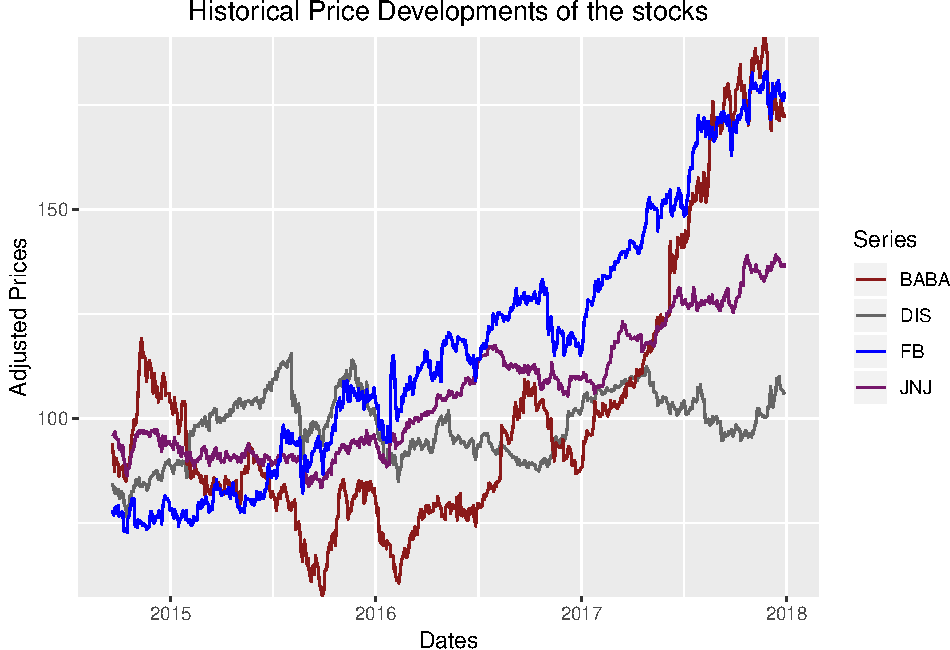
\includegraphics{Markowitz_Research_Me_files/figure-latex/unnamed-chunk-2-1.pdf}

\begin{Shaded}
\begin{Highlighting}[]
\KeywordTok{head}\NormalTok{(prices,}\DecValTok{10}\NormalTok{)}
\end{Highlighting}
\end{Shaded}

\begin{verbatim}
##                 DIS  BABA      JNJ    FB
## 2014-09-19 84.29720 93.89 96.16410 77.91
## 2014-09-22 83.17931 89.89 96.06615 76.80
## 2014-09-23 82.26636 87.17 95.69215 78.29
## 2014-09-24 83.32836 90.57 96.74294 78.54
## 2014-09-25 82.04281 88.92 95.37157 77.22
## 2014-09-26 82.66695 90.46 95.37157 78.79
## 2014-09-29 82.75080 88.75 94.87290 79.00
## 2014-09-30 82.93709 88.85 94.91740 79.04
## 2014-10-01 81.50249 86.10 92.87820 76.55
## 2014-10-02 80.85040 87.06 92.47746 77.08
\end{verbatim}

\subsubsection{Dygraphs}\label{dygraphs}

\begin{Shaded}
\begin{Highlighting}[]
\CommentTok{#plot dygraph from package dygraphs}
\CommentTok{#dygraph(prices,main = "Prices of stocks",xlab = "Dates",ylab = "Prices")}
\NormalTok{## Uncomment abive to see dygraphs}
\CommentTok{# basic time series plot with range slider underneath}
\CommentTok{#dygraph(prices) %>% dyRangeSelector()}
\NormalTok{## uncomment above to see dygraphs}
\end{Highlighting}
\end{Shaded}

\subsubsection{Chart series for the
stocks}\label{chart-series-for-the-stocks}

\begin{Shaded}
\begin{Highlighting}[]
\KeywordTok{chartSeries}\NormalTok{(BABA)}
\end{Highlighting}
\end{Shaded}

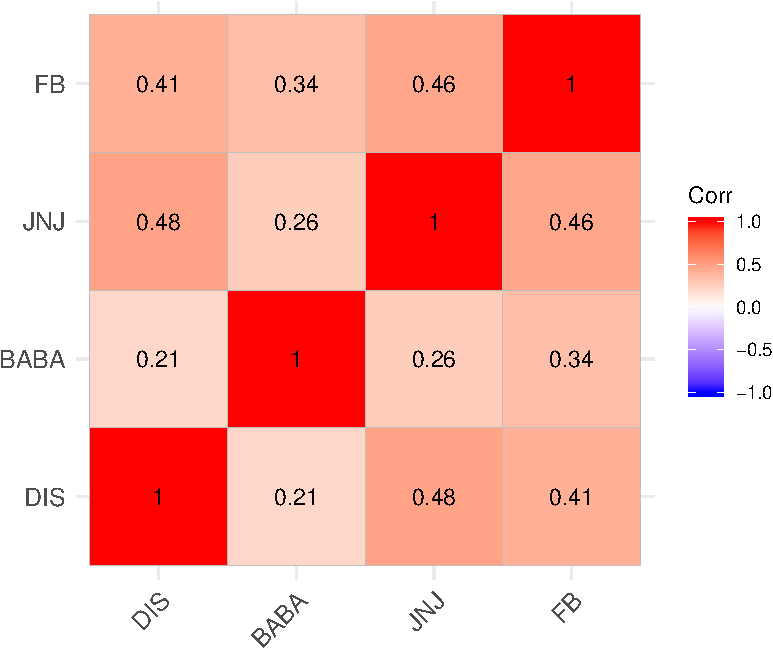
\includegraphics{Markowitz_Research_Me_files/figure-latex/unnamed-chunk-4-1.pdf}

\begin{Shaded}
\begin{Highlighting}[]
\KeywordTok{chartSeries}\NormalTok{(FB)}
\end{Highlighting}
\end{Shaded}

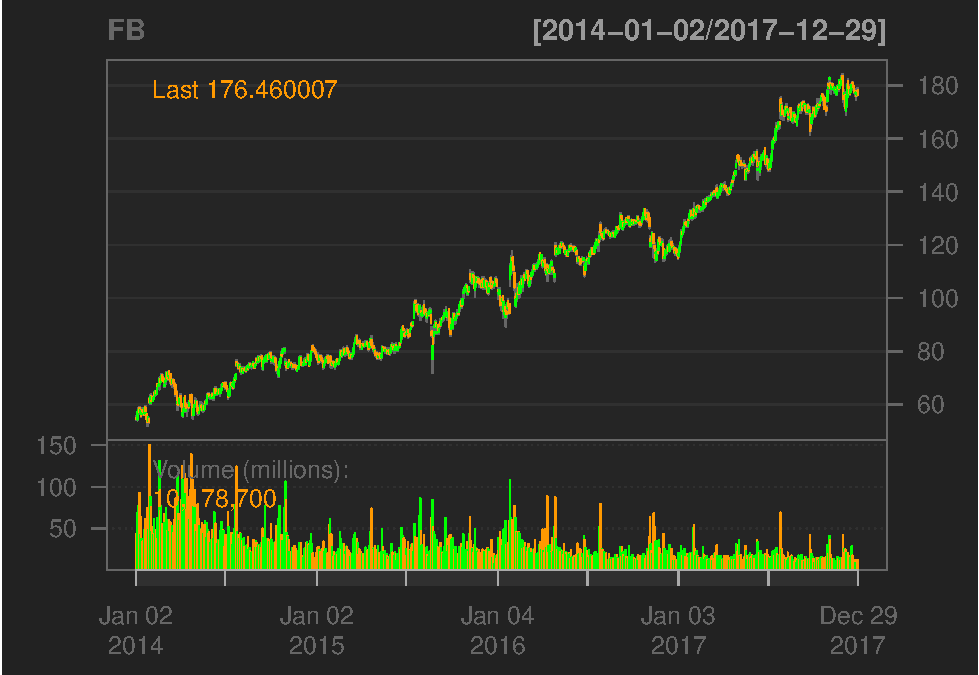
\includegraphics{Markowitz_Research_Me_files/figure-latex/unnamed-chunk-4-2.pdf}

\begin{Shaded}
\begin{Highlighting}[]
\KeywordTok{chartSeries}\NormalTok{(DIS)}
\end{Highlighting}
\end{Shaded}

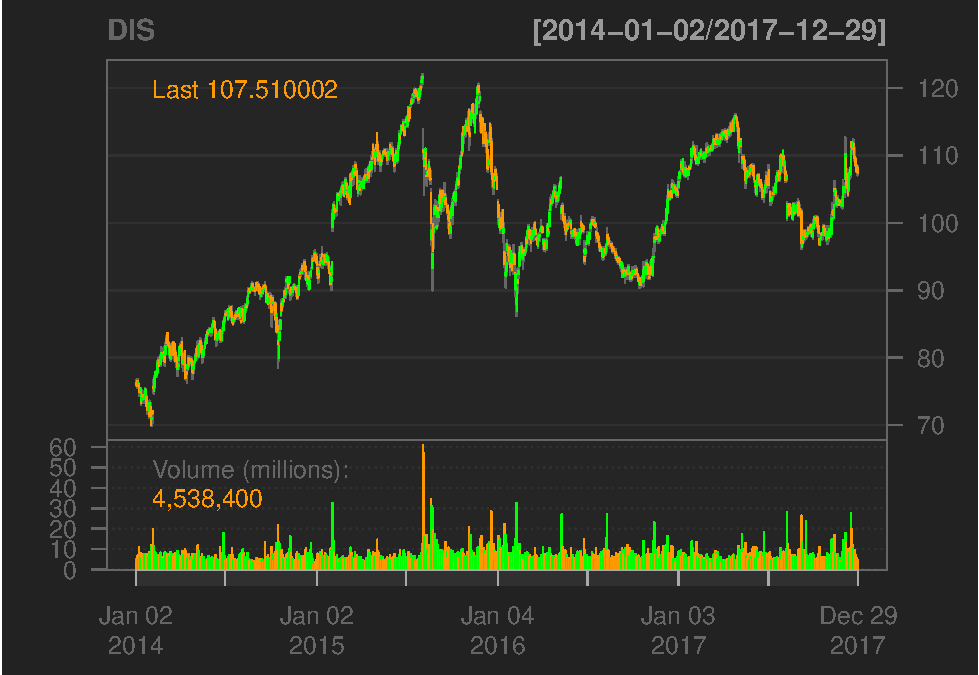
\includegraphics{Markowitz_Research_Me_files/figure-latex/unnamed-chunk-4-3.pdf}

\begin{Shaded}
\begin{Highlighting}[]
\KeywordTok{chartSeries}\NormalTok{(JNJ)}
\end{Highlighting}
\end{Shaded}

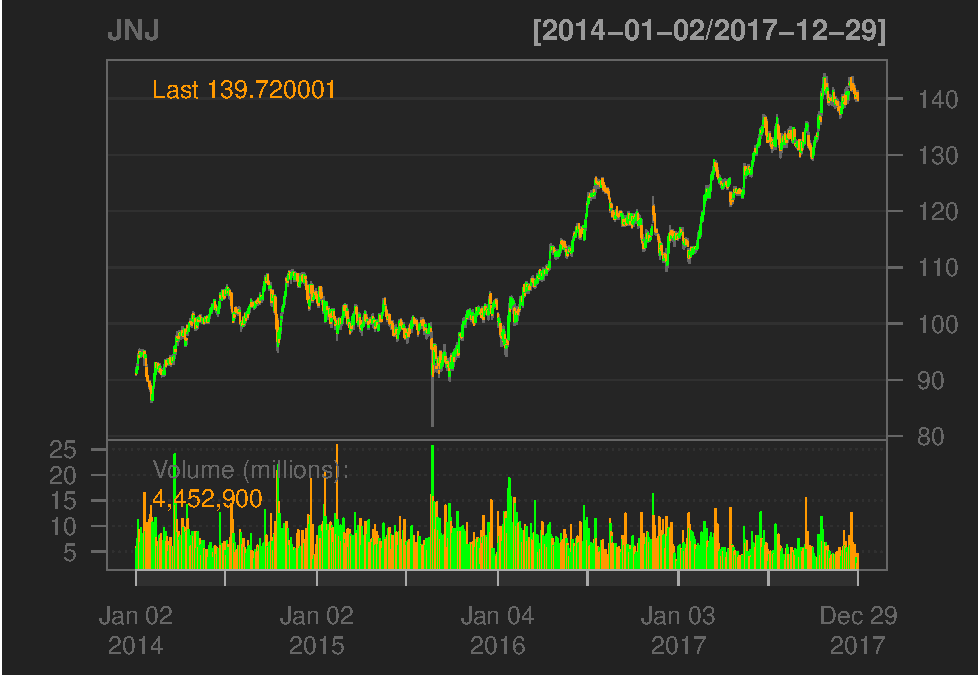
\includegraphics{Markowitz_Research_Me_files/figure-latex/unnamed-chunk-4-4.pdf}

\subsubsection{Corrplot for 2014-2016}\label{corrplot-for-2014-2016}

\begin{Shaded}
\begin{Highlighting}[]
\NormalTok{begin1 =}\StringTok{ "2014-01-01"}
\NormalTok{end1 =}\StringTok{ "2016-01-01"}
\NormalTok{stocks =}\StringTok{ }\KeywordTok{c}\NormalTok{(}\StringTok{"DIS"}\NormalTok{,}\StringTok{"BABA"}\NormalTok{,}\StringTok{"JNJ"}\NormalTok{,}\StringTok{"FB"}\NormalTok{)}
\KeywordTok{suppressMessages}\NormalTok{(}\KeywordTok{getSymbols}\NormalTok{(stocks,}\DataTypeTok{from=}\NormalTok{begin1, }\DataTypeTok{to =}\NormalTok{ end1))}
\end{Highlighting}
\end{Shaded}

\begin{verbatim}
## [1] "DIS"  "BABA" "JNJ"  "FB"
\end{verbatim}

\begin{Shaded}
\begin{Highlighting}[]
\NormalTok{prices1 =}\StringTok{ }\KeywordTok{na.omit}\NormalTok{(}\KeywordTok{merge}\NormalTok{(}\KeywordTok{Ad}\NormalTok{(DIS),}\KeywordTok{Ad}\NormalTok{(BABA),}\KeywordTok{Ad}\NormalTok{(JNJ),}\KeywordTok{Ad}\NormalTok{(FB)))}
\KeywordTok{names}\NormalTok{(prices1) <-}\StringTok{ }\KeywordTok{c}\NormalTok{(}\StringTok{"DIS"}\NormalTok{,}\StringTok{"BABA"}\NormalTok{,}\StringTok{"JNJ"}\NormalTok{,}\StringTok{"FB"}\NormalTok{)}
\NormalTok{prices1<-}\StringTok{ }\KeywordTok{as.matrix}\NormalTok{(prices1)}
\NormalTok{Xi1 =}\StringTok{ }\DecValTok{365}\OperatorTok{*}\KeywordTok{diff}\NormalTok{(}\KeywordTok{log}\NormalTok{(prices1))}
\NormalTok{corr1 <-}\StringTok{ }\KeywordTok{round}\NormalTok{(}\KeywordTok{cor}\NormalTok{(Xi1), }\DecValTok{3}\NormalTok{)}
\KeywordTok{head}\NormalTok{(corr1[, }\DecValTok{1}\OperatorTok{:}\DecValTok{4}\NormalTok{])}
\end{Highlighting}
\end{Shaded}

\begin{verbatim}
##        DIS  BABA   JNJ    FB
## DIS  1.000 0.211 0.484 0.410
## BABA 0.211 1.000 0.259 0.336
## JNJ  0.484 0.259 1.000 0.458
## FB   0.410 0.336 0.458 1.000
\end{verbatim}

\begin{Shaded}
\begin{Highlighting}[]
\KeywordTok{ggcorrplot}\NormalTok{(corr1,}\DataTypeTok{lab =} \OtherTok{TRUE}\NormalTok{)}
\end{Highlighting}
\end{Shaded}

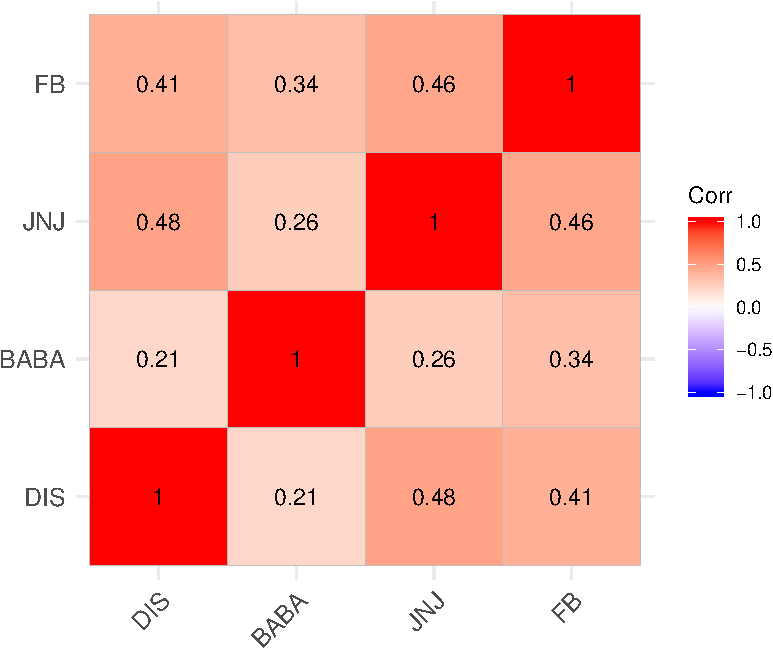
\includegraphics{Markowitz_Research_Me_files/figure-latex/unnamed-chunk-5-1.pdf}

\subsubsection{Corrplot for 2016-2018}\label{corrplot-for-2016-2018}

\begin{Shaded}
\begin{Highlighting}[]
\NormalTok{begin2 =}\StringTok{ "2016-01-01"}
\NormalTok{end2 =}\StringTok{ "2018-01-01"}
\NormalTok{stocks =}\StringTok{ }\KeywordTok{c}\NormalTok{(}\StringTok{"DIS"}\NormalTok{,}\StringTok{"BABA"}\NormalTok{,}\StringTok{"JNJ"}\NormalTok{,}\StringTok{"FB"}\NormalTok{)}
\KeywordTok{suppressMessages}\NormalTok{(}\KeywordTok{getSymbols}\NormalTok{(stocks,}\DataTypeTok{from=}\NormalTok{begin2, }\DataTypeTok{to =}\NormalTok{ end2))}
\end{Highlighting}
\end{Shaded}

\begin{verbatim}
## [1] "DIS"  "BABA" "JNJ"  "FB"
\end{verbatim}

\begin{Shaded}
\begin{Highlighting}[]
\NormalTok{prices2 =}\StringTok{ }\KeywordTok{na.omit}\NormalTok{(}\KeywordTok{merge}\NormalTok{(}\KeywordTok{Ad}\NormalTok{(DIS),}\KeywordTok{Ad}\NormalTok{(BABA),}\KeywordTok{Ad}\NormalTok{(JNJ),}\KeywordTok{Ad}\NormalTok{(FB))) }
\KeywordTok{names}\NormalTok{(prices2) <-}\StringTok{ }\KeywordTok{c}\NormalTok{(}\StringTok{"DIS"}\NormalTok{,}\StringTok{"BABA"}\NormalTok{,}\StringTok{"JNJ"}\NormalTok{,}\StringTok{"FB"}\NormalTok{)}
\NormalTok{prices2<-}\StringTok{ }\KeywordTok{as.matrix}\NormalTok{(prices2)}
\NormalTok{Xi2 =}\StringTok{ }\DecValTok{365}\OperatorTok{*}\KeywordTok{diff}\NormalTok{(}\KeywordTok{log}\NormalTok{(prices2))}
\NormalTok{corr2 <-}\StringTok{ }\KeywordTok{round}\NormalTok{(}\KeywordTok{cor}\NormalTok{(Xi2), }\DecValTok{3}\NormalTok{)}
\KeywordTok{head}\NormalTok{(corr2[, }\DecValTok{1}\OperatorTok{:}\DecValTok{4}\NormalTok{])}
\end{Highlighting}
\end{Shaded}

\begin{verbatim}
##        DIS  BABA   JNJ    FB
## DIS  1.000 0.162 0.149 0.152
## BABA 0.162 1.000 0.164 0.355
## JNJ  0.149 0.164 1.000 0.209
## FB   0.152 0.355 0.209 1.000
\end{verbatim}

\begin{Shaded}
\begin{Highlighting}[]
\KeywordTok{ggcorrplot}\NormalTok{(corr2,}\DataTypeTok{lab =} \OtherTok{TRUE}\NormalTok{)}
\end{Highlighting}
\end{Shaded}

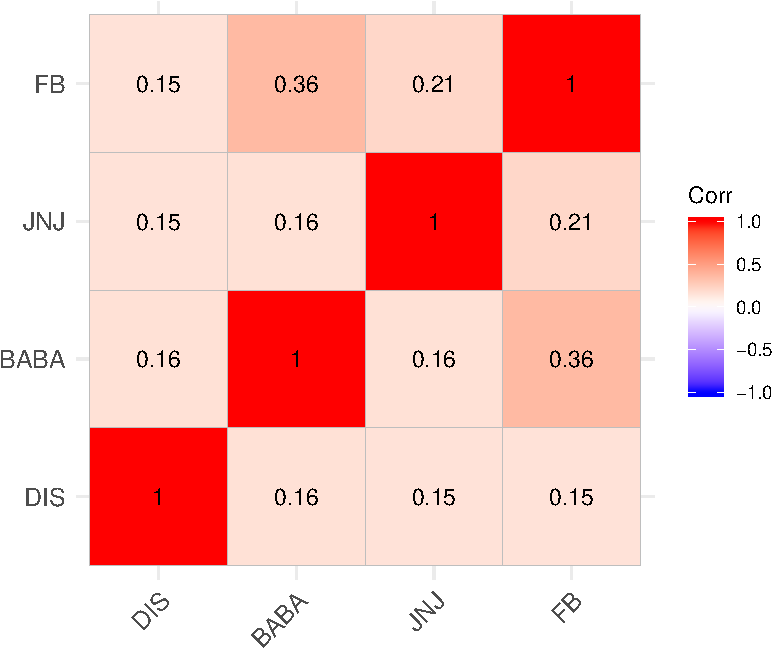
\includegraphics{Markowitz_Research_Me_files/figure-latex/unnamed-chunk-6-1.pdf}

\subsubsection{Matrix plot for scaled prices for the
data}\label{matrix-plot-for-scaled-prices-for-the-data}

\begin{Shaded}
\begin{Highlighting}[]
\CommentTok{#Scaled prices}
\NormalTok{prices.scaled =}\StringTok{ }\NormalTok{prices_matrix}
\NormalTok{m =}\StringTok{ }\KeywordTok{dim}\NormalTok{(prices_matrix)}
\ControlFlowTok{for}\NormalTok{ (k }\ControlFlowTok{in}\NormalTok{ (}\DecValTok{1}\OperatorTok{:}\NormalTok{m[}\DecValTok{2}\NormalTok{]))\{}
\NormalTok{  prices.scaled[,k] =}\StringTok{ }\NormalTok{prices.scaled[,k]}\OperatorTok{/}\NormalTok{prices.scaled[}\DecValTok{1}\NormalTok{,k]}
\NormalTok{\}}

\KeywordTok{matplot}\NormalTok{(prices.scaled,}\DataTypeTok{type=}\StringTok{'l'}\NormalTok{,}\DataTypeTok{xaxt=}\StringTok{"n"}\NormalTok{,}\DataTypeTok{lwd =}\DecValTok{1}\NormalTok{,}
        \DataTypeTok{col=}\DecValTok{1}\OperatorTok{:}\NormalTok{m[}\DecValTok{2}\NormalTok{],}\DataTypeTok{xlab=}\StringTok{"Dates"}\NormalTok{,}\DataTypeTok{ylab=}\StringTok{"Scaled Prices"}\NormalTok{)}
\KeywordTok{legend}\NormalTok{(}\StringTok{"topleft"}\NormalTok{, stocks, }\DataTypeTok{col=}\DecValTok{1}\OperatorTok{:}\NormalTok{m[}\DecValTok{2}\NormalTok{],}\DataTypeTok{lwd=}\DecValTok{1}\NormalTok{)}
\end{Highlighting}
\end{Shaded}

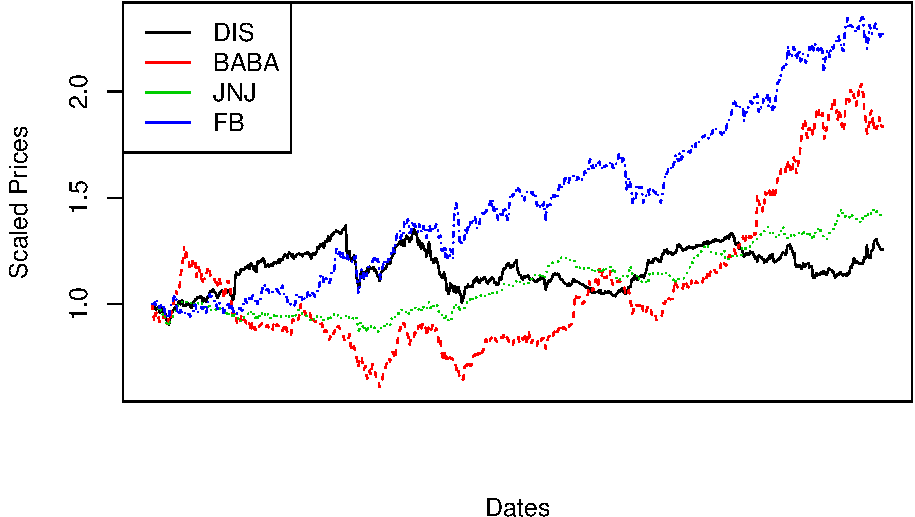
\includegraphics{Markowitz_Research_Me_files/figure-latex/unnamed-chunk-7-1.pdf}

\subsubsection{Matrix of annualized returns,skewness and
kurtosis}\label{matrix-of-annualized-returnsskewness-and-kurtosis}

\begin{Shaded}
\begin{Highlighting}[]
\CommentTok{#Matrix of Annualized Returns}
\NormalTok{Xi =}\StringTok{ }\DecValTok{365}\OperatorTok{*}\KeywordTok{diff}\NormalTok{(}\KeywordTok{log}\NormalTok{(prices_matrix))}
\CommentTok{#round(Xi*100,2) #Annualized returns in percentages}
\CommentTok{# skewness and kurtosis from the package psych}
\KeywordTok{skew}\NormalTok{(Xi)}
\end{Highlighting}
\end{Shaded}

\begin{verbatim}
## [1] -0.7823843  0.2267734  0.1575834  0.6631494
\end{verbatim}

\begin{Shaded}
\begin{Highlighting}[]
\KeywordTok{kurtosi}\NormalTok{(Xi)}
\end{Highlighting}
\end{Shaded}

\begin{verbatim}
##       DIS      BABA       JNJ        FB 
##  9.333801  3.495925  2.692699 10.718660
\end{verbatim}

\subsubsection{Expected annualied returns and variance(biased and
unbiased)}\label{expected-annualied-returns-and-variancebiased-and-unbiased}

\begin{Shaded}
\begin{Highlighting}[]
\NormalTok{dim_xi =}\StringTok{ }\KeywordTok{dim}\NormalTok{(Xi)}
\NormalTok{n =}\StringTok{ }\NormalTok{dim_xi[}\DecValTok{1}\NormalTok{]}
\NormalTok{j =}\StringTok{ }\NormalTok{dim_xi[}\DecValTok{2}\NormalTok{]}
\CommentTok{#first moment: expected annulized returns }
\NormalTok{returns =}\StringTok{ }\KeywordTok{colMeans}\NormalTok{(Xi)}
\NormalTok{returns}
\end{Highlighting}
\end{Shaded}

\begin{verbatim}
##       DIS      BABA       JNJ        FB 
## 0.1005307 0.2686097 0.1532568 0.3612616
\end{verbatim}

\begin{Shaded}
\begin{Highlighting}[]
\KeywordTok{apply}\NormalTok{(}\DataTypeTok{X=}\NormalTok{Xi, }\DataTypeTok{MARGIN=}\DecValTok{2}\NormalTok{,}\DataTypeTok{FUN =}\NormalTok{ mean)}\OperatorTok{*}\DecValTok{100}
\end{Highlighting}
\end{Shaded}

\begin{verbatim}
##      DIS     BABA      JNJ       FB 
## 10.05307 26.86097 15.32568 36.12616
\end{verbatim}

\begin{Shaded}
\begin{Highlighting}[]
\CommentTok{#Second moment : variance }
\NormalTok{(}\KeywordTok{apply}\NormalTok{(}\DataTypeTok{X=}\NormalTok{Xi, }\DataTypeTok{MARGIN =} \DecValTok{2}\NormalTok{, }\DataTypeTok{FUN =}\NormalTok{ var)) }\CommentTok{#biased }
\end{Highlighting}
\end{Shaded}

\begin{verbatim}
##      DIS     BABA      JNJ       FB 
## 18.27308 50.49671 10.76208 31.17938
\end{verbatim}

\begin{Shaded}
\begin{Highlighting}[]
\NormalTok{(}\KeywordTok{apply}\NormalTok{(}\DataTypeTok{X=}\NormalTok{Xi, }\DataTypeTok{MARGIN =} \DecValTok{2}\NormalTok{, }\DataTypeTok{FUN =}\NormalTok{ var) }\OperatorTok{*}\StringTok{ }\NormalTok{(n}\OperatorTok{-}\DecValTok{1}\NormalTok{)}\OperatorTok{/}\NormalTok{n)}\OperatorTok{*}\DecValTok{100} \CommentTok{#unbiased}
\end{Highlighting}
\end{Shaded}

\begin{verbatim}
##      DIS     BABA      JNJ       FB 
## 1825.096 5043.557 1074.905 3114.163
\end{verbatim}

\begin{Shaded}
\begin{Highlighting}[]
\CommentTok{#standard deviation}
\NormalTok{(}\KeywordTok{apply}\NormalTok{(}\DataTypeTok{X=}\NormalTok{Xi, }\DataTypeTok{MARGIN =} \DecValTok{2}\NormalTok{, }\DataTypeTok{FUN =}\NormalTok{ sd))}\OperatorTok{*}\DecValTok{100} \CommentTok{#biased }
\end{Highlighting}
\end{Shaded}

\begin{verbatim}
##      DIS     BABA      JNJ       FB 
## 427.4703 710.6103 328.0561 558.3850
\end{verbatim}

\begin{Shaded}
\begin{Highlighting}[]
\NormalTok{(}\KeywordTok{apply}\NormalTok{(}\DataTypeTok{X=}\NormalTok{Xi, }\DataTypeTok{MARGIN =} \DecValTok{2}\NormalTok{, }\DataTypeTok{FUN =}\NormalTok{ sd) }\OperatorTok{*}\StringTok{ }\NormalTok{(n}\OperatorTok{-}\DecValTok{1}\NormalTok{)}\OperatorTok{/}\NormalTok{n)}\OperatorTok{*}\DecValTok{100} \CommentTok{#unbiased}
\end{Highlighting}
\end{Shaded}

\begin{verbatim}
##      DIS     BABA      JNJ       FB 
## 426.9527 709.7500 327.6589 557.7090
\end{verbatim}

\subsubsection{Covariance matrix}\label{covariance-matrix}

From below, we should note that the covariance matrix is symmetric and
is also positive definite. Also, the diagonal of the covariance matrix
are the variances of the stocks. And since it is symmetric, then also
the covariance matrix is also invertible.

\begin{Shaded}
\begin{Highlighting}[]
\KeywordTok{cov}\NormalTok{(Xi)}
\end{Highlighting}
\end{Shaded}

\begin{verbatim}
##            DIS      BABA       JNJ        FB
## DIS  18.273082  5.788963  4.657648  6.717097
## BABA  5.788963 50.496707  5.157152 13.846795
## JNJ   4.657648  5.157152 10.762081  6.118848
## FB    6.717097 13.846795  6.118848 31.179377
\end{verbatim}

\begin{Shaded}
\begin{Highlighting}[]
\KeywordTok{diag}\NormalTok{(}\KeywordTok{cov}\NormalTok{(Xi))}\OperatorTok{*}\DecValTok{100} \CommentTok{#biased}
\end{Highlighting}
\end{Shaded}

\begin{verbatim}
##      DIS     BABA      JNJ       FB 
## 1827.308 5049.671 1076.208 3117.938
\end{verbatim}

\begin{Shaded}
\begin{Highlighting}[]
\NormalTok{(}\KeywordTok{cov}\NormalTok{(Xi)}\OperatorTok{*}\NormalTok{(n}\OperatorTok{-}\DecValTok{1}\NormalTok{)}\OperatorTok{/}\NormalTok{n)}
\end{Highlighting}
\end{Shaded}

\begin{verbatim}
##            DIS      BABA       JNJ        FB
## DIS  18.250959  5.781954  4.652009  6.708965
## BABA  5.781954 50.435573  5.150908 13.830031
## JNJ   4.652009  5.150908 10.749052  6.111440
## FB    6.708965 13.830031  6.111440 31.141630
\end{verbatim}

\begin{Shaded}
\begin{Highlighting}[]
\KeywordTok{diag}\NormalTok{(}\KeywordTok{cov}\NormalTok{(Xi)}\OperatorTok{*}\NormalTok{(n}\OperatorTok{-}\DecValTok{1}\NormalTok{)}\OperatorTok{/}\NormalTok{n) }\CommentTok{#unbiased}
\end{Highlighting}
\end{Shaded}

\begin{verbatim}
##      DIS     BABA      JNJ       FB 
## 18.25096 50.43557 10.74905 31.14163
\end{verbatim}

\subsection{CAPM solution.}\label{capm-solution.}

\subsubsection{Covariance Matrix}\label{covariance-matrix-1}

\begin{Shaded}
\begin{Highlighting}[]
\NormalTok{Covar =}\StringTok{ }\KeywordTok{cov}\NormalTok{(Xi)}\OperatorTok{*}\NormalTok{(n}\OperatorTok{-}\DecValTok{1}\NormalTok{)}\OperatorTok{/}\NormalTok{n}
\NormalTok{inv_C =}\StringTok{ }\KeywordTok{solve}\NormalTok{(Covar)}
\NormalTok{Covar}
\end{Highlighting}
\end{Shaded}

\begin{verbatim}
##            DIS      BABA       JNJ        FB
## DIS  18.250959  5.781954  4.652009  6.708965
## BABA  5.781954 50.435573  5.150908 13.830031
## JNJ   4.652009  5.150908 10.749052  6.111440
## FB    6.708965 13.830031  6.111440 31.141630
\end{verbatim}

\subsubsection{Correlation of the
assets}\label{correlation-of-the-assets}

\begin{Shaded}
\begin{Highlighting}[]
\NormalTok{corr <-}\StringTok{ }\KeywordTok{round}\NormalTok{(}\KeywordTok{cor}\NormalTok{(Xi), }\DecValTok{3}\NormalTok{)}
\KeywordTok{head}\NormalTok{(corr[, }\DecValTok{1}\OperatorTok{:}\DecValTok{4}\NormalTok{])}
\end{Highlighting}
\end{Shaded}

\begin{verbatim}
##        DIS  BABA   JNJ    FB
## DIS  1.000 0.191 0.332 0.281
## BABA 0.191 1.000 0.221 0.349
## JNJ  0.332 0.221 1.000 0.334
## FB   0.281 0.349 0.334 1.000
\end{verbatim}

\begin{Shaded}
\begin{Highlighting}[]
\KeywordTok{ggcorrplot}\NormalTok{(corr,}\DataTypeTok{lab =} \OtherTok{TRUE}\NormalTok{)}
\end{Highlighting}
\end{Shaded}

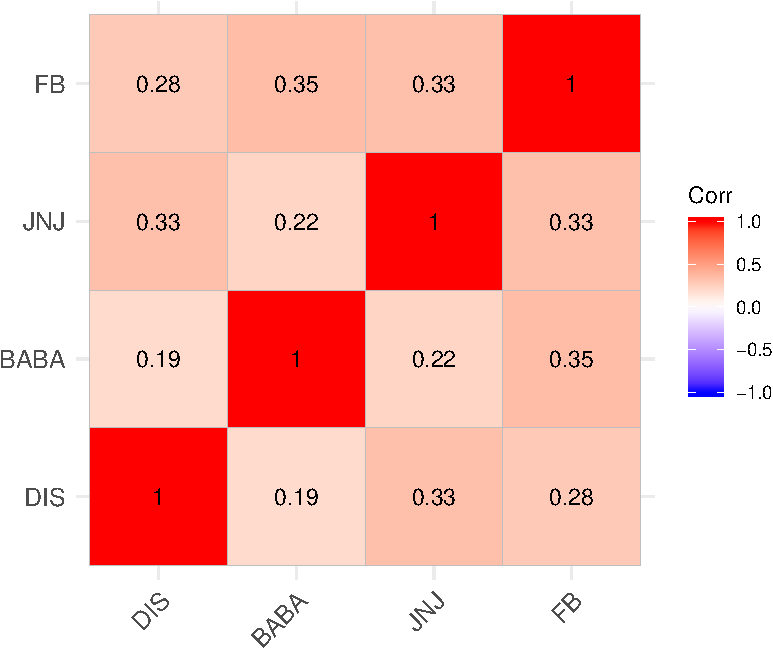
\includegraphics{Markowitz_Research_Me_files/figure-latex/unnamed-chunk-12-1.pdf}

\begin{Shaded}
\begin{Highlighting}[]
\CommentTok{# correlation chart}
\KeywordTok{chart.Correlation}\NormalTok{(Xi)}
\end{Highlighting}
\end{Shaded}

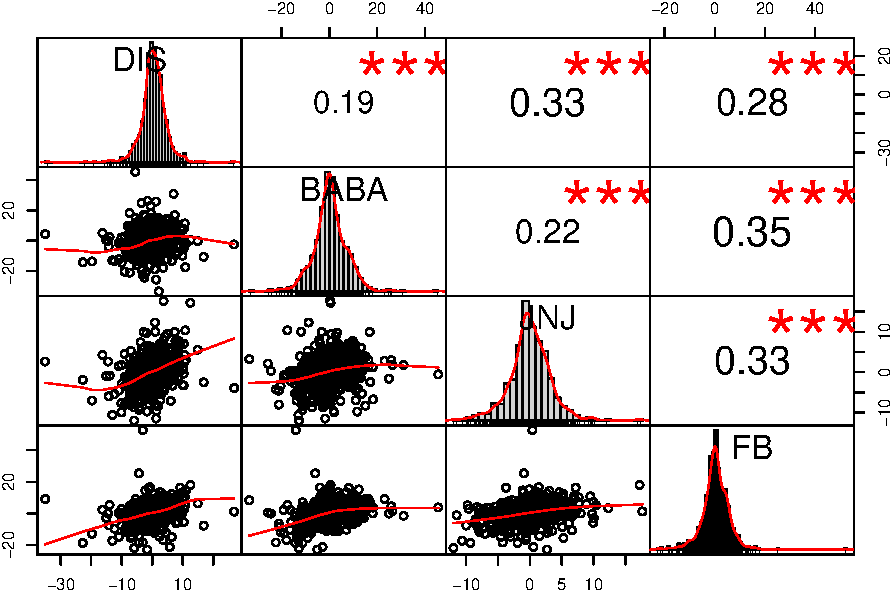
\includegraphics{Markowitz_Research_Me_files/figure-latex/unnamed-chunk-12-2.pdf}

\subsubsection{Inverse of the covariance
matrix}\label{inverse-of-the-covariance-matrix}

Generally, we know that the inverse of a positive definite symmetric
matrix is also symmetric. Clearly, the inverse of the covariance matrix
below is alo symmetric.

\begin{Shaded}
\begin{Highlighting}[]
\KeywordTok{round}\NormalTok{(inv_C,}\DecValTok{2}\NormalTok{)}
\end{Highlighting}
\end{Shaded}

\begin{verbatim}
##        DIS  BABA   JNJ    FB
## DIS   0.06  0.00 -0.02 -0.01
## BABA  0.00  0.02  0.00 -0.01
## JNJ  -0.02  0.00  0.11 -0.02
## FB   -0.01 -0.01 -0.02  0.04
\end{verbatim}

\begin{Shaded}
\begin{Highlighting}[]
\KeywordTok{round}\NormalTok{(inv_C}\OperatorTok{*}\DecValTok{100}\NormalTok{,}\DecValTok{2}\NormalTok{)}
\end{Highlighting}
\end{Shaded}

\begin{verbatim}
##        DIS  BABA   JNJ    FB
## DIS   6.43 -0.29 -2.17 -0.83
## BABA -0.29  2.30 -0.49 -0.87
## JNJ  -2.17 -0.49 11.35 -1.54
## FB   -0.83 -0.87 -1.54  4.08
\end{verbatim}

\subsubsection{A,B,C and D values}\label{abc-and-d-values}

\begin{Shaded}
\begin{Highlighting}[]
\NormalTok{ones =}\StringTok{ }\KeywordTok{rep}\NormalTok{(}\DecValTok{1}\NormalTok{,j)}
\NormalTok{A =}\StringTok{ }\KeywordTok{as.numeric}\NormalTok{(returns}\OperatorTok\StringTok{ }\NormalTok{inv_C }\OperatorTok\StringTok{ }\NormalTok{returns)}
\NormalTok{B =}\StringTok{ }\KeywordTok{as.numeric}\NormalTok{(returns}\OperatorTok\StringTok{ }\NormalTok{inv_C }\OperatorTok\StringTok{ }\NormalTok{ones )}
\NormalTok{C =}\StringTok{ }\KeywordTok{as.numeric}\NormalTok{(ones }\OperatorTok\StringTok{ }\NormalTok{inv_C }\OperatorTok\StringTok{ }\NormalTok{ones )}
\NormalTok{D =}\StringTok{ }\NormalTok{A}\OperatorTok{*}\NormalTok{C}\OperatorTok{-}\NormalTok{B}\OperatorTok{*}\NormalTok{B}
\NormalTok{first <-}\StringTok{ }\NormalTok{C}\OperatorTok{/}\NormalTok{D }\OperatorTok{*}\StringTok{ }\NormalTok{inv_C }\OperatorTok\StringTok{ }\NormalTok{returns}
\NormalTok{first2 <-}\StringTok{ }\NormalTok{B}\OperatorTok{/}\NormalTok{D }\OperatorTok{*}\StringTok{ }\NormalTok{inv_C }\OperatorTok\StringTok{ }\NormalTok{returns}
\NormalTok{first3 <-}\StringTok{ }\NormalTok{A}\OperatorTok{/}\NormalTok{D }\OperatorTok{*}\StringTok{ }\NormalTok{inv_C }\OperatorTok\StringTok{ }\NormalTok{ones}
\NormalTok{first4 <-}\StringTok{ }\NormalTok{B}\OperatorTok{/}\NormalTok{D }\OperatorTok{*}\StringTok{ }\NormalTok{inv_C }\OperatorTok\StringTok{ }\NormalTok{ones}
\NormalTok{first }\OperatorTok{-}\StringTok{ }\NormalTok{first4}
\end{Highlighting}
\end{Shaded}

\begin{verbatim}
##            [,1]
## DIS  -2.7756963
## BABA  0.4695406
## JNJ  -1.5374357
## FB    3.8435914
\end{verbatim}

\begin{Shaded}
\begin{Highlighting}[]
\NormalTok{first3 }\OperatorTok{-}\StringTok{ }\NormalTok{first2}
\end{Highlighting}
\end{Shaded}

\begin{verbatim}
##             [,1]
## DIS   0.71164775
## BABA -0.01911337
## JNJ   0.85326827
## FB   -0.54580265
\end{verbatim}

\subsubsection{Efficient Markowitz
portfolio}\label{efficient-markowitz-portfolio}

\begin{Shaded}
\begin{Highlighting}[]
\NormalTok{mu =}\StringTok{ }\KeywordTok{seq}\NormalTok{(}\DataTypeTok{from=}\FloatTok{0.00}\NormalTok{,}\DataTypeTok{to =} \FloatTok{0.3}\NormalTok{,}\DataTypeTok{by=}\FloatTok{0.01}\NormalTok{)}
\NormalTok{ml =}\StringTok{ }\KeywordTok{length}\NormalTok{(mu)}
\NormalTok{xm =}\StringTok{ }\KeywordTok{matrix}\NormalTok{(}\DataTypeTok{nrow =}\NormalTok{ j, }\DataTypeTok{ncol=}\NormalTok{ml)}
\ControlFlowTok{for}\NormalTok{ (k }\ControlFlowTok{in} \DecValTok{1}\OperatorTok{:}\NormalTok{ml)\{}
\NormalTok{  xm[,k]=}\StringTok{ }\NormalTok{A}\OperatorTok{*}\NormalTok{inv_C}\OperatorTok\NormalTok{ones}\OperatorTok{-}\StringTok{ }\NormalTok{B}\OperatorTok{*}\NormalTok{inv_C}\OperatorTok\NormalTok{returns}\OperatorTok{+}\StringTok{ }\NormalTok{mu[k]}\OperatorTok{*}\NormalTok{(C}\OperatorTok{*}\NormalTok{inv_C}\OperatorTok\NormalTok{returns }\OperatorTok{-}\NormalTok{B}\OperatorTok{*}\NormalTok{inv_C}\OperatorTok\NormalTok{ones) }
\NormalTok{\}}
\NormalTok{xm =}\StringTok{ }\NormalTok{xm}\OperatorTok{/}\NormalTok{D}
\KeywordTok{colSums}\NormalTok{(xm)}
\end{Highlighting}
\end{Shaded}

\begin{verbatim}
##  [1] 1 1 1 1 1 1 1 1 1 1 1 1 1 1 1 1 1 1 1 1 1 1 1 1 1 1 1 1 1 1 1
\end{verbatim}

we know that
\(\text{standard deviation} = \sqrt{\frac{\mu^2 * c - 2* \mu *b + a}{d}}\)
where \(d = a*c - b^2\) and so we can see the relationship between
standard deviation and returns for our data in the following figure:

\begin{Shaded}
\begin{Highlighting}[]
\NormalTok{standarddev =}\StringTok{ }\KeywordTok{sqrt}\NormalTok{((mu}\OperatorTok{*}\NormalTok{mu}\OperatorTok{*}\NormalTok{C}\OperatorTok{-}\DecValTok{2}\OperatorTok{*}\NormalTok{mu}\OperatorTok{*}\NormalTok{B}\OperatorTok{+}\NormalTok{A)}\OperatorTok{/}\NormalTok{D)}
\NormalTok{var =}\StringTok{ }\NormalTok{mu}\OperatorTok{*}\NormalTok{mu}\OperatorTok{*}\NormalTok{C}\OperatorTok{-}\DecValTok{2}\OperatorTok{*}\NormalTok{mu}\OperatorTok{*}\NormalTok{B}\OperatorTok{+}\NormalTok{A}\OperatorTok{/}\NormalTok{D}
\NormalTok{min_mu =}\StringTok{ }\NormalTok{B}\OperatorTok{/}\NormalTok{C }\CommentTok{#minimum expected return}
\NormalTok{min_var =}\StringTok{ }\KeywordTok{sqrt}\NormalTok{(}\DecValTok{1}\OperatorTok{/}\NormalTok{C) }\CommentTok{#minimum standard dviation}
\NormalTok{sharpeRatio =}\StringTok{ }\NormalTok{min_mu}\OperatorTok{/}\NormalTok{min_var }\CommentTok{# sharpe ratio}
\NormalTok{Expe_port =}\StringTok{ }\NormalTok{sharpeRatio}\OperatorTok{*}\NormalTok{standarddev }\CommentTok{# portfolio returns for CML}
\KeywordTok{plot}\NormalTok{(mu,standarddev,}\DataTypeTok{type=}\StringTok{"l"}\NormalTok{,}\DataTypeTok{main=}\StringTok{"Standard deviation of the optimal portfolio in dependence of mu"}\NormalTok{)}
\end{Highlighting}
\end{Shaded}

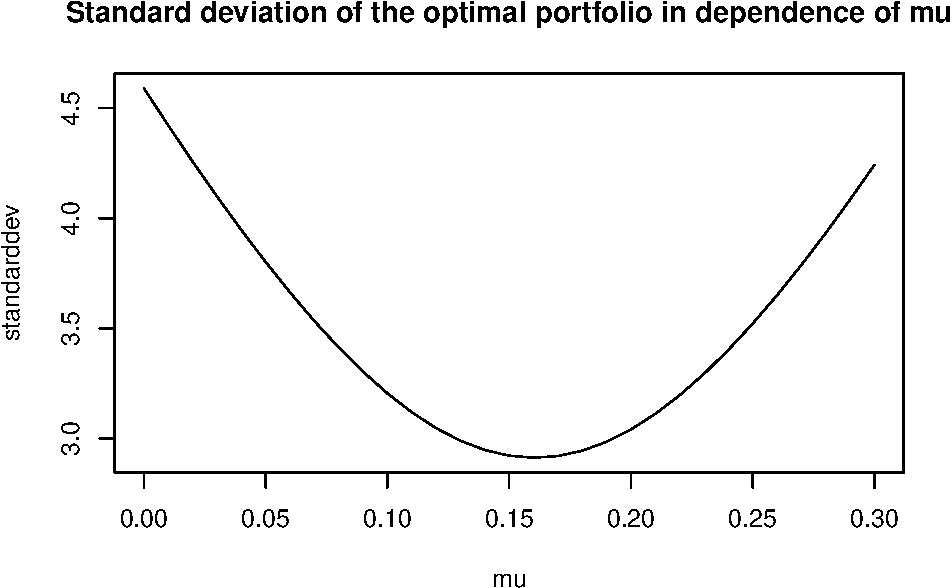
\includegraphics{Markowitz_Research_Me_files/figure-latex/unnamed-chunk-16-1.pdf}

\begin{Shaded}
\begin{Highlighting}[]
\KeywordTok{plot}\NormalTok{(standarddev,mu,}\DataTypeTok{type =} \StringTok{"l"}\NormalTok{, }\DataTypeTok{main =} \StringTok{"Efficient frontier"}\NormalTok{)}
\KeywordTok{points}\NormalTok{(min_var,min_mu,}\DataTypeTok{pch =} \DecValTok{8}\NormalTok{, }\DataTypeTok{col =} \StringTok{"red"}\NormalTok{,}\DataTypeTok{cex =} \DecValTok{1}\NormalTok{)}
\KeywordTok{text}\NormalTok{(}\FloatTok{3.5}\NormalTok{,min_mu,}\KeywordTok{expression}\NormalTok{(}\StringTok{"Min variance point, mu = 0.1605,var = 2.9124"}\NormalTok{))}
\end{Highlighting}
\end{Shaded}

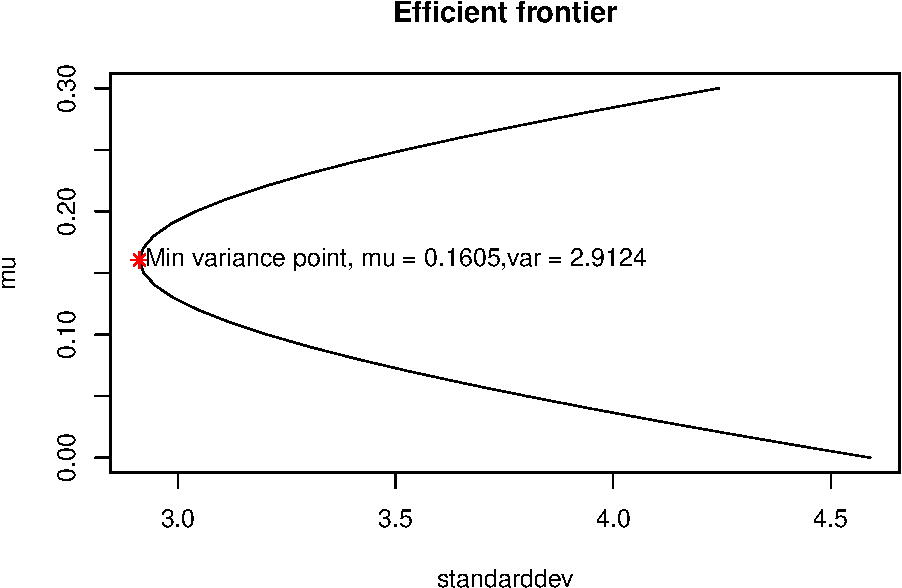
\includegraphics{Markowitz_Research_Me_files/figure-latex/unnamed-chunk-16-2.pdf}

The portfolio with the smallest variance from our combinations is given
by \(\mu = \frac{b}{c} = 0.1604767 = 16.05\%\) which is clear from the
diagram and the corresponding standard deviation is given by
\(\sigma= \sqrt{\frac{1}{C}} = 2.912357 = 291.24\%\).

\subsubsection{Asset allocation figure.}\label{asset-allocation-figure.}

\begin{Shaded}
\begin{Highlighting}[]
\KeywordTok{matplot}\NormalTok{(mu,}\KeywordTok{t}\NormalTok{(xm),}\DataTypeTok{type=}\StringTok{'l'}\NormalTok{,}\DataTypeTok{col=}\DecValTok{1}\OperatorTok{:}\NormalTok{j,}\DataTypeTok{lty=}\DecValTok{1}\OperatorTok{:}\NormalTok{j,}\DataTypeTok{ylab=}\StringTok{"x*"}\NormalTok{,}\DataTypeTok{main=}\StringTok{"Asset Allocation"}\NormalTok{)}
\KeywordTok{legend}\NormalTok{(}\StringTok{"topright"}\NormalTok{, stocks,}\DataTypeTok{col=}\DecValTok{1}\OperatorTok{:}\NormalTok{j, }\DataTypeTok{lty=}\DecValTok{1}\OperatorTok{:}\NormalTok{j,}\DataTypeTok{bty=}\StringTok{"n"}\NormalTok{,}\DataTypeTok{lwd=}\DecValTok{1}\NormalTok{)}
\end{Highlighting}
\end{Shaded}

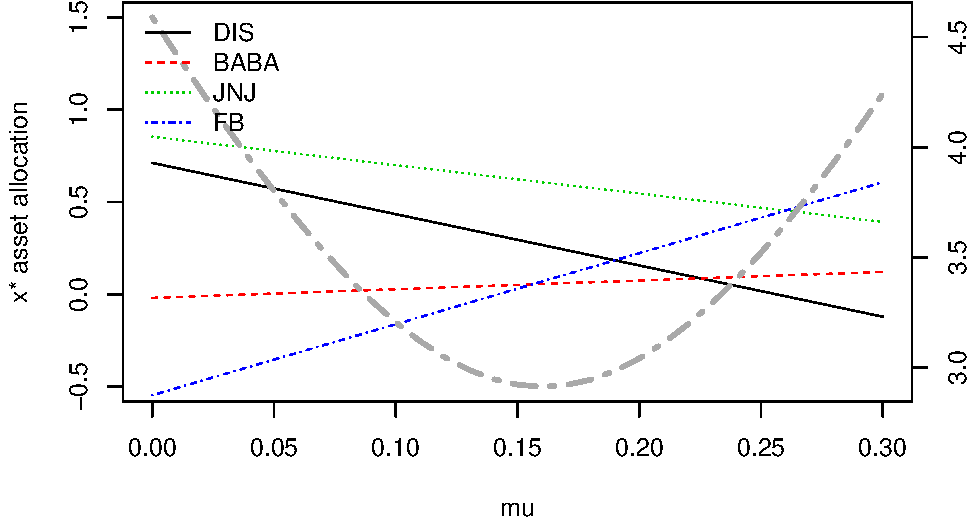
\includegraphics{Markowitz_Research_Me_files/figure-latex/unnamed-chunk-17-1.pdf}

\begin{Shaded}
\begin{Highlighting}[]
\CommentTok{# Or we can plot a stacked barplot which will appear a bit better than above}
\KeywordTok{library}\NormalTok{(reshape2)}
\NormalTok{asset_alloc <-}\StringTok{ }\KeywordTok{data.frame}\NormalTok{(mu,}\KeywordTok{t}\NormalTok{(xm))}
\KeywordTok{names}\NormalTok{(asset_alloc) <-}\StringTok{ }\KeywordTok{c}\NormalTok{(}\StringTok{"mu"}\NormalTok{,}\StringTok{"DIS"}\NormalTok{,}\StringTok{"BABA"}\NormalTok{,}\StringTok{"JNJ"}\NormalTok{,}\StringTok{"FB"}\NormalTok{)}
\NormalTok{asset_alloc <-}\StringTok{ }\KeywordTok{melt}\NormalTok{(asset_alloc, }\DataTypeTok{id =} \StringTok{"mu"}\NormalTok{)}
\KeywordTok{names}\NormalTok{(asset_alloc) <-}\StringTok{ }\KeywordTok{c}\NormalTok{(}\StringTok{"mu"}\NormalTok{,}\StringTok{"Stocks"}\NormalTok{,}\StringTok{"Allocation"}\NormalTok{)}
\KeywordTok{ggplot}\NormalTok{() }\OperatorTok{+}\StringTok{ }\KeywordTok{geom_bar}\NormalTok{(}\KeywordTok{aes}\NormalTok{(}\DataTypeTok{y =}\NormalTok{ Allocation, }\DataTypeTok{x =}\NormalTok{ mu, }\DataTypeTok{fill =}\NormalTok{ Stocks), }\DataTypeTok{data =}\NormalTok{ asset_alloc, }\DataTypeTok{stat=}\StringTok{"identity"}\NormalTok{)}\OperatorTok{+}
\StringTok{  }\KeywordTok{scale_fill_manual}\NormalTok{(}\StringTok{"Stocks"}\NormalTok{,}\DataTypeTok{values =}
                      \KeywordTok{c}\NormalTok{(}\StringTok{"FB"}\NormalTok{=}\StringTok{"#0000FF"}\NormalTok{,}\StringTok{"JNJ"}\NormalTok{=}\StringTok{"#00FF00"}\NormalTok{,}\StringTok{"BABA"}\NormalTok{=}\StringTok{"#FF0000"}\NormalTok{,}\StringTok{"DIS"}\NormalTok{=}\StringTok{"#454545"}\NormalTok{)) }
\end{Highlighting}
\end{Shaded}

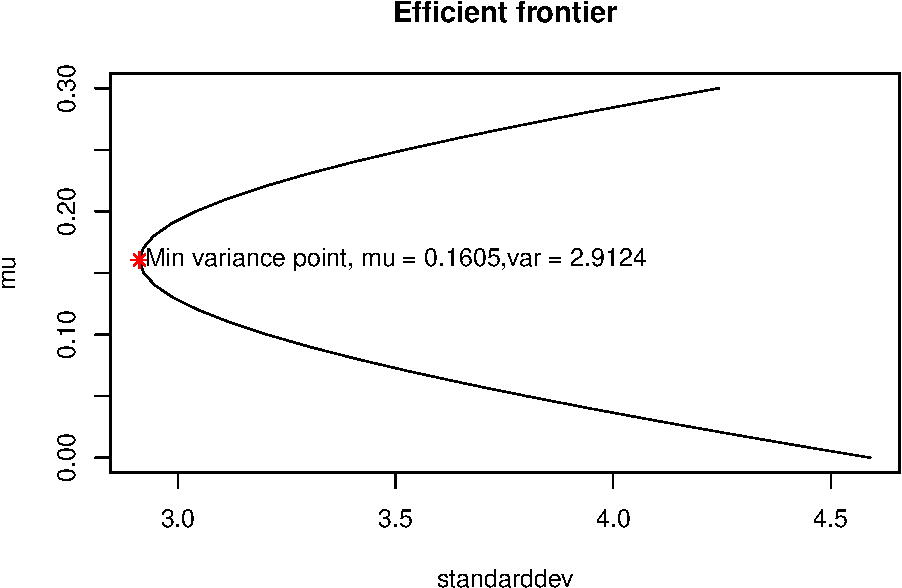
\includegraphics{Markowitz_Research_Me_files/figure-latex/unnamed-chunk-17-2.pdf}

\subsubsection{Combined asset allocation and standard
deviation}\label{combined-asset-allocation-and-standard-deviation}

\begin{Shaded}
\begin{Highlighting}[]
\KeywordTok{plot}\NormalTok{(mu,}\KeywordTok{t}\NormalTok{(xm[}\DecValTok{1}\NormalTok{,]),}\DataTypeTok{ylim=}\KeywordTok{c}\NormalTok{(}\OperatorTok{-}\FloatTok{0.5}\NormalTok{,}\FloatTok{1.5}\NormalTok{),}\DataTypeTok{type=}\StringTok{'l'}\NormalTok{,}\DataTypeTok{col=}\DecValTok{1}\NormalTok{,}\DataTypeTok{lty=}\DecValTok{1}\NormalTok{,}\DataTypeTok{ylab=}\StringTok{"x* asset allocation"}\NormalTok{)}
\ControlFlowTok{for}\NormalTok{ (k }\ControlFlowTok{in} \DecValTok{2}\OperatorTok{:}\NormalTok{j) }\KeywordTok{lines}\NormalTok{(mu,}\KeywordTok{t}\NormalTok{(xm[k,]),}\DataTypeTok{type=}\StringTok{'l'}\NormalTok{,}\DataTypeTok{col=}\NormalTok{k,}\DataTypeTok{lty=}\NormalTok{k)}
\KeywordTok{par}\NormalTok{(}\DataTypeTok{new=}\OtherTok{TRUE}\NormalTok{)}
\KeywordTok{plot}\NormalTok{(mu, standarddev,}\DataTypeTok{type=}\StringTok{"l"}\NormalTok{,}\DataTypeTok{col=}\StringTok{"darkgray"}\NormalTok{,}\DataTypeTok{lwd=}\DecValTok{3}\NormalTok{,}\DataTypeTok{lty=}\DecValTok{6}\NormalTok{,}\DataTypeTok{xaxt=}\StringTok{"n"}\NormalTok{,}\DataTypeTok{yaxt=}\StringTok{"n"}\NormalTok{,}\DataTypeTok{xlab=}\StringTok{""}\NormalTok{,}\DataTypeTok{ylab=}\StringTok{""}\NormalTok{)}
\KeywordTok{axis}\NormalTok{(}\DecValTok{4}\NormalTok{)}
\KeywordTok{mtext}\NormalTok{(}\StringTok{"sd(x*(mu))"}\NormalTok{,}\DataTypeTok{side=}\DecValTok{4}\NormalTok{,}\DataTypeTok{line=}\DecValTok{3}\NormalTok{,}\DataTypeTok{col=}\StringTok{"darkgray"}\NormalTok{)}
\KeywordTok{legend}\NormalTok{(}\StringTok{"topleft"}\NormalTok{, }\KeywordTok{c}\NormalTok{(stocks), }\DataTypeTok{col=}\KeywordTok{c}\NormalTok{(}\DecValTok{1}\OperatorTok{:}\NormalTok{j), }\DataTypeTok{lty=}\DecValTok{1}\OperatorTok{:}\NormalTok{(j),}\DataTypeTok{bty=}\StringTok{"n"}\NormalTok{,}\DataTypeTok{lwd=}\KeywordTok{rep}\NormalTok{(}\DecValTok{1}\NormalTok{,j))}
\end{Highlighting}
\end{Shaded}

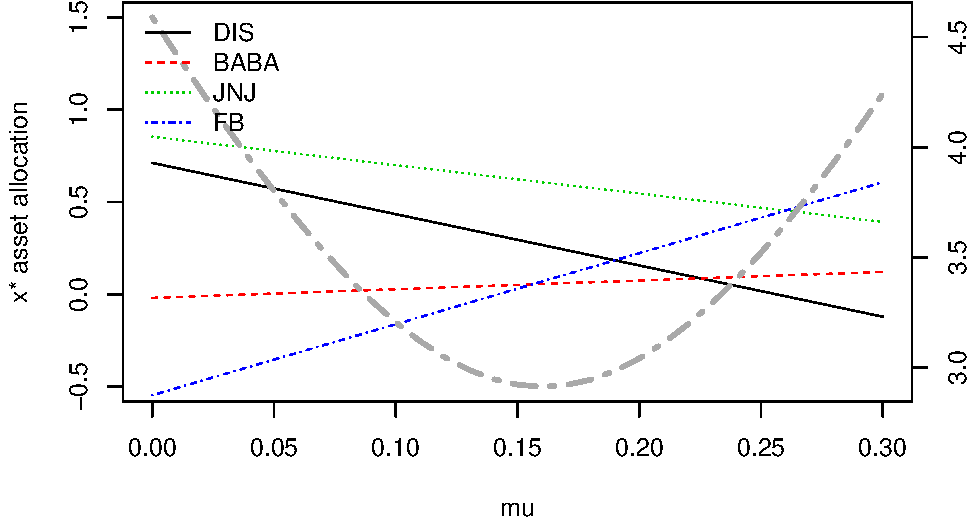
\includegraphics{Markowitz_Research_Me_files/figure-latex/unnamed-chunk-18-1.pdf}

\subsection{PART 2}\label{part-2}

We are going to use the package \textbf{fPortfolio} in this part to
study the Markowitz model.

\subsubsection{Makowitz model using fPortfolio package and
others}\label{makowitz-model-using-fportfolio-package-and-others}

I will be using the package ``fPortfolio'' to study the Markowitz model.
This package is specifically geared towards portfolio optimization.

In order to construct a minimum variance portfolio, we will need 3
things:

\begin{itemize}
\tightlist
\item
  Historical Returns
\item
  Historical volatility
\item
  Covariance matrix and correlation matrix
\end{itemize}

We are going to consider the following 4 stocks during the period of
2010-01-01 to 2018-01-01:

\begin{itemize}
\tightlist
\item
  DIS
\item
  BABA
\item
  JNJ
\item
  FB
\end{itemize}

\subsubsection{Obtaining data using the quantmod
package}\label{obtaining-data-using-the-quantmod-package}

We will also be creating a time series object to allow us plot the
Efficient frontier. We will use the ``\textbf{getSymbols}'' function
from \textbf{quantmod} to be able to gather the prices for the stocks
which we will use to calculate returns and convert the data into a time
series object.

\begin{Shaded}
\begin{Highlighting}[]
\NormalTok{tickers <-}\StringTok{ }\KeywordTok{c}\NormalTok{(}\StringTok{"DIS"}\NormalTok{, }\StringTok{"BABA"}\NormalTok{, }\StringTok{"JNJ"}\NormalTok{, }\StringTok{"FB"}\NormalTok{)}
\CommentTok{#Calculate Returns: Daily}
\NormalTok{portfolioPrices <-}\StringTok{ }\OtherTok{NULL}
\ControlFlowTok{for}\NormalTok{ (Ticker }\ControlFlowTok{in}\NormalTok{ tickers)}
\NormalTok{  portfolioPrices <-}\StringTok{ }\KeywordTok{cbind}\NormalTok{(portfolioPrices,}
                           \KeywordTok{suppressMessages}\NormalTok{(}\KeywordTok{getSymbols}\NormalTok{(Ticker,}\DataTypeTok{from=}\StringTok{"2014-01-01"}\NormalTok{,}
                                      \DataTypeTok{to=}\StringTok{"2018-01-01"}\NormalTok{,}\DataTypeTok{auto.assign=}\OtherTok{FALSE}\NormalTok{)[,}\DecValTok{4}\NormalTok{]))}
\NormalTok{portfolioPrices <-}\StringTok{ }\NormalTok{portfolioPrices[}\KeywordTok{apply}\NormalTok{(portfolioPrices,}\DecValTok{1}\NormalTok{,}\ControlFlowTok{function}\NormalTok{(x) }\KeywordTok{all}\NormalTok{(}\OperatorTok{!}\KeywordTok{is.na}\NormalTok{(x))),]}
\KeywordTok{colnames}\NormalTok{(portfolioPrices) <-}\StringTok{ }\NormalTok{tickers}
\CommentTok{#Calculate Returns: Daily RoC}
\NormalTok{portfolioReturns <-}\StringTok{ }\KeywordTok{na.omit}\NormalTok{(}\KeywordTok{ROC}\NormalTok{(portfolioPrices, }\DataTypeTok{type=}\StringTok{"discrete"}\NormalTok{))}\OperatorTok{*}\DecValTok{365}
\KeywordTok{colnames}\NormalTok{(portfolioReturns) <-}\StringTok{ }\NormalTok{tickers}
\CommentTok{#Plot of the returns developments of the above data}
\KeywordTok{ggplot}\NormalTok{(portfolioReturns, }\KeywordTok{aes}\NormalTok{(}\DataTypeTok{x =} \KeywordTok{index}\NormalTok{(portfolioReturns))) }\OperatorTok{+}
\StringTok{  }\KeywordTok{geom_line}\NormalTok{(}\KeywordTok{aes}\NormalTok{(}\DataTypeTok{y =}\NormalTok{ portfolioReturns}\OperatorTok{$}\NormalTok{DIS,}\DataTypeTok{color =} \StringTok{"DIS"}\NormalTok{)) }\OperatorTok{+}\StringTok{ }
\StringTok{  }\KeywordTok{ggtitle}\NormalTok{(}\StringTok{"Historical portfolio returns of the stocks"}\NormalTok{) }\OperatorTok{+}
\StringTok{  }\KeywordTok{geom_line}\NormalTok{(}\KeywordTok{aes}\NormalTok{(}\DataTypeTok{y =}\NormalTok{ portfolioReturns}\OperatorTok{$}\NormalTok{BABA, }\DataTypeTok{color =} \StringTok{"BABA"}\NormalTok{)) }\OperatorTok{+}\StringTok{ }
\StringTok{  }\KeywordTok{geom_line}\NormalTok{(}\KeywordTok{aes}\NormalTok{(}\DataTypeTok{y =}\NormalTok{ portfolioReturns}\OperatorTok{$}\NormalTok{JNJ, }\DataTypeTok{color =} \StringTok{"JNJ"}\NormalTok{)) }\OperatorTok{+}
\StringTok{  }\KeywordTok{geom_line}\NormalTok{(}\KeywordTok{aes}\NormalTok{(}\DataTypeTok{y =}\NormalTok{ portfolioReturns}\OperatorTok{$}\NormalTok{FB, }\DataTypeTok{color =} \StringTok{"FB"}\NormalTok{)) }\OperatorTok{+}
\StringTok{  }\KeywordTok{xlab}\NormalTok{(}\StringTok{"Dates"}\NormalTok{) }\OperatorTok{+}\StringTok{ }\KeywordTok{ylab}\NormalTok{(}\StringTok{"Adjusted Prices"}\NormalTok{) }\OperatorTok{+}
\StringTok{  }\KeywordTok{theme}\NormalTok{(}\DataTypeTok{plot.title =} \KeywordTok{element_text}\NormalTok{(}\DataTypeTok{hjust =} \FloatTok{0.5}\NormalTok{), }\DataTypeTok{panel.border =} \KeywordTok{element_blank}\NormalTok{()) }\OperatorTok{+}
\StringTok{  }\KeywordTok{scale_y_continuous}\NormalTok{(}\DataTypeTok{expand =} \KeywordTok{c}\NormalTok{(}\DecValTok{0}\NormalTok{,}\DecValTok{0}\NormalTok{)) }\OperatorTok{+}
\StringTok{  }\KeywordTok{scale_colour_manual}\NormalTok{(}\StringTok{"Stocks"}\NormalTok{,}\DataTypeTok{values=}\KeywordTok{c}\NormalTok{(}\StringTok{"DIS"}\NormalTok{=}\StringTok{"#FF0000"}\NormalTok{,}\StringTok{"BABA"}\NormalTok{=}\StringTok{"#00FF00"}\NormalTok{,}
                                        \StringTok{"JNJ"}\NormalTok{=}\StringTok{"#0000FF"}\NormalTok{,}\StringTok{"FB"}\NormalTok{=}\StringTok{"#454545"}\NormalTok{))}
\end{Highlighting}
\end{Shaded}

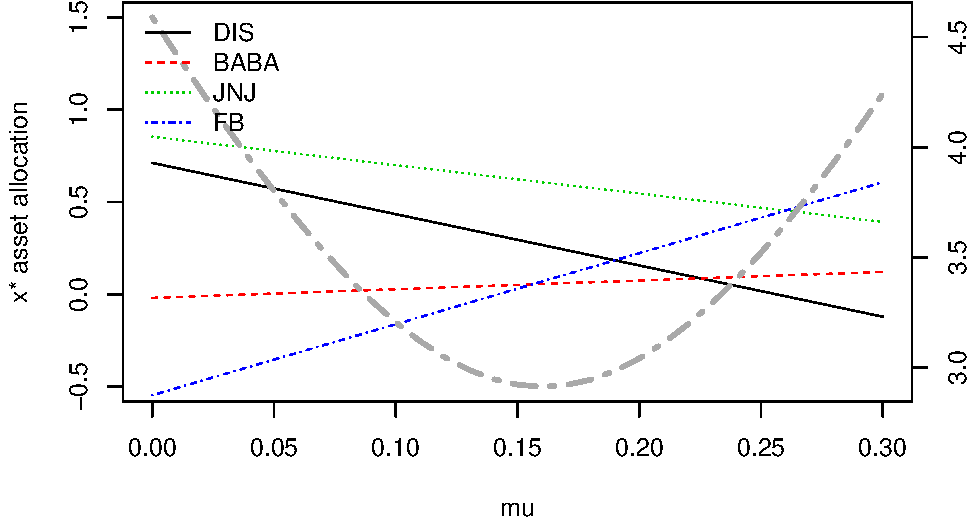
\includegraphics{Markowitz_Research_Me_files/figure-latex/unnamed-chunk-19-1.pdf}

\begin{Shaded}
\begin{Highlighting}[]
\KeywordTok{plot.zoo}\NormalTok{(portfolioReturns,}\DataTypeTok{col =} \KeywordTok{c}\NormalTok{(}\StringTok{"DIS"}\NormalTok{=}\StringTok{"#FF0000"}\NormalTok{,}\StringTok{"BABA"}\NormalTok{=}\StringTok{"#00FF00"}\NormalTok{,}
                                        \StringTok{"FB"}\NormalTok{=}\StringTok{"#0000FF"}\NormalTok{,}\StringTok{"JNJ"}\NormalTok{=}\StringTok{"#454545"}\NormalTok{))}
\end{Highlighting}
\end{Shaded}

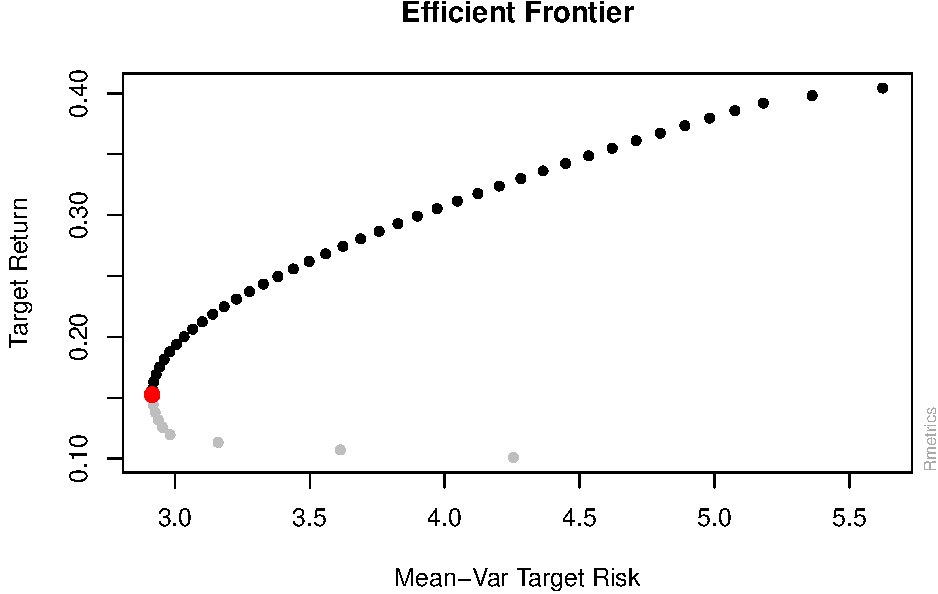
\includegraphics{Markowitz_Research_Me_files/figure-latex/unnamed-chunk-19-2.pdf}

\begin{Shaded}
\begin{Highlighting}[]
\NormalTok{portfolioReturns <-}\StringTok{ }\KeywordTok{as.timeSeries}\NormalTok{(portfolioReturns)}
\CommentTok{#Checking on the dimension of the portfolio prices}
\KeywordTok{dim}\NormalTok{(portfolioPrices)}
\end{Highlighting}
\end{Shaded}

\begin{verbatim}
## [1] 827   4
\end{verbatim}

\begin{Shaded}
\begin{Highlighting}[]
\KeywordTok{dim}\NormalTok{(portfolioReturns)}
\end{Highlighting}
\end{Shaded}

\begin{verbatim}
## [1] 826   4
\end{verbatim}

\begin{Shaded}
\begin{Highlighting}[]
\KeywordTok{head}\NormalTok{(portfolioPrices)}
\end{Highlighting}
\end{Shaded}

\begin{verbatim}
##              DIS  BABA    JNJ    FB
## 2014-09-19 90.49 93.89 107.99 77.91
## 2014-09-22 89.29 89.89 107.88 76.80
## 2014-09-23 88.31 87.17 107.46 78.29
## 2014-09-24 89.45 90.57 108.64 78.54
## 2014-09-25 88.07 88.92 107.10 77.22
## 2014-09-26 88.74 90.46 107.10 78.79
\end{verbatim}

\begin{Shaded}
\begin{Highlighting}[]
\KeywordTok{head}\NormalTok{(portfolioReturns)}
\end{Highlighting}
\end{Shaded}

\begin{verbatim}
## GMT
##                  DIS       BABA        JNJ         FB
## 2014-09-22 -4.840302 -15.550112 -0.3717971 -5.2002355
## 2014-09-23 -4.006060 -11.044614 -1.4210166  7.0813704
## 2014-09-24  4.711807  14.236558  4.0080030  1.1655384
## 2014-09-25 -5.631067  -6.649561 -5.1739725 -6.1344537
## 2014-09-26  2.776760   6.321417  0.0000000  7.4210048
## 2014-09-29  0.370199  -6.899731 -1.9084865  0.9728345
\end{verbatim}

\begin{Shaded}
\begin{Highlighting}[]
\CommentTok{#Plot of the price developments of the above data}
\KeywordTok{ggplot}\NormalTok{(portfolioPrices, }\KeywordTok{aes}\NormalTok{(}\DataTypeTok{x =} \KeywordTok{index}\NormalTok{(portfolioPrices))) }\OperatorTok{+}
\StringTok{  }\KeywordTok{geom_line}\NormalTok{(}\KeywordTok{aes}\NormalTok{(}\DataTypeTok{y =}\NormalTok{ portfolioPrices}\OperatorTok{$}\NormalTok{DIS,}\DataTypeTok{color =} \StringTok{"DIS"}\NormalTok{)) }\OperatorTok{+}\StringTok{ }
\StringTok{  }\KeywordTok{ggtitle}\NormalTok{(}\StringTok{"Historical Portfolio Prices of the stocks"}\NormalTok{) }\OperatorTok{+}
\StringTok{  }\KeywordTok{geom_line}\NormalTok{(}\KeywordTok{aes}\NormalTok{(}\DataTypeTok{y =}\NormalTok{ portfolioPrices}\OperatorTok{$}\NormalTok{BABA, }\DataTypeTok{color =} \StringTok{"BABA"}\NormalTok{)) }\OperatorTok{+}\StringTok{ }
\StringTok{  }\KeywordTok{geom_line}\NormalTok{(}\KeywordTok{aes}\NormalTok{(}\DataTypeTok{y =}\NormalTok{ portfolioPrices}\OperatorTok{$}\NormalTok{JNJ, }\DataTypeTok{color =} \StringTok{"JNJ"}\NormalTok{)) }\OperatorTok{+}
\StringTok{  }\KeywordTok{geom_line}\NormalTok{(}\KeywordTok{aes}\NormalTok{(}\DataTypeTok{y =}\NormalTok{ portfolioPrices}\OperatorTok{$}\NormalTok{FB, }\DataTypeTok{color =} \StringTok{"FB"}\NormalTok{)) }\OperatorTok{+}
\StringTok{  }\KeywordTok{xlab}\NormalTok{(}\StringTok{"Dates"}\NormalTok{) }\OperatorTok{+}\StringTok{ }\KeywordTok{ylab}\NormalTok{(}\StringTok{"Adjusted Prices"}\NormalTok{) }\OperatorTok{+}
\StringTok{  }\KeywordTok{theme}\NormalTok{(}\DataTypeTok{plot.title =} \KeywordTok{element_text}\NormalTok{(}\DataTypeTok{hjust =} \FloatTok{0.5}\NormalTok{), }\DataTypeTok{panel.border =} \KeywordTok{element_blank}\NormalTok{()) }\OperatorTok{+}
\StringTok{  }\KeywordTok{scale_y_continuous}\NormalTok{(}\DataTypeTok{expand =} \KeywordTok{c}\NormalTok{(}\DecValTok{0}\NormalTok{,}\DecValTok{0}\NormalTok{)) }\OperatorTok{+}
\StringTok{  }\KeywordTok{scale_colour_manual}\NormalTok{(}\StringTok{"Stocks"}\NormalTok{,}\DataTypeTok{values=}\KeywordTok{c}\NormalTok{(}\StringTok{"DIS"}\NormalTok{=}\StringTok{"#FF0000"}\NormalTok{,}\StringTok{"BABA"}\NormalTok{=}\StringTok{"#00FF00"}\NormalTok{,}
                                        \StringTok{"JNJ"}\NormalTok{=}\StringTok{"#454545"}\NormalTok{,}\StringTok{"FB"}\NormalTok{=}\StringTok{"#0000FF"}\NormalTok{))}
\end{Highlighting}
\end{Shaded}

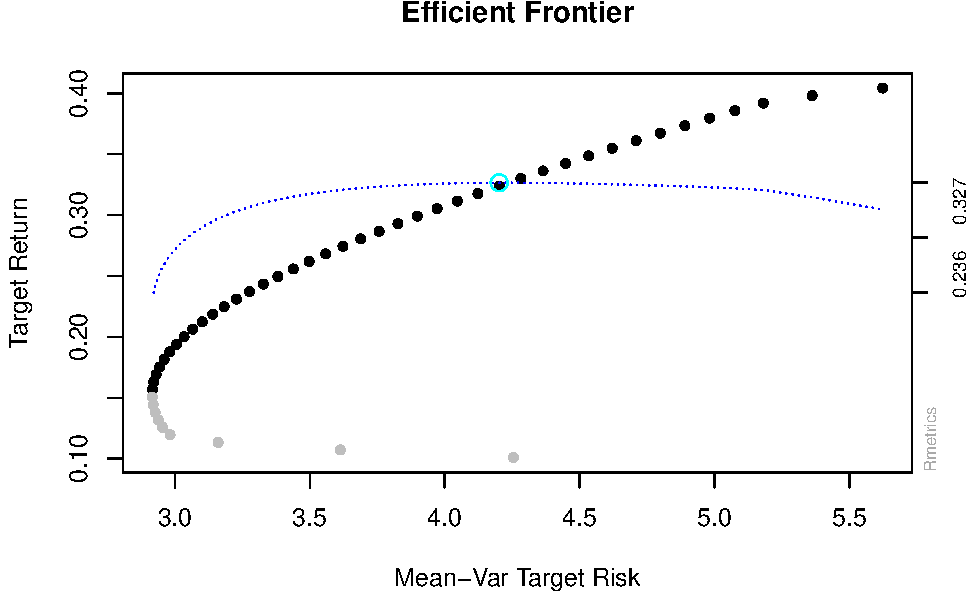
\includegraphics{Markowitz_Research_Me_files/figure-latex/unnamed-chunk-19-3.pdf}

\subsubsection{Portfolio frontier
calculation}\label{portfolio-frontier-calculation}

I will now calculate and plot the efficient frontier by using the
function " \textbf{portfolioFrontier}``. I will also output the
covariance matrix and correlation matrix for our portfolio of assets. We
can also extract certain portfolios sucsh as the Minimun Variance
Portfolio or Maximum Return Portfolio.

We will also examine the weights of each point on the frontier
graphically. We will also annualize the data and plot the risk returns
on a scatter plot also. Also, we will plot the Sharpe Ratio of each
point on the frontier on a scatter graph.

We will also see the Value-at-risk and conditional value-at-risk of the
portfolio returns at different levels

\begin{Shaded}
\begin{Highlighting}[]
\CommentTok{# calculate the efficient frontier}
\NormalTok{effFrontier <-}\StringTok{ }\KeywordTok{portfolioFrontier}\NormalTok{(portfolioReturns,}
                                 \DataTypeTok{constraints =} \StringTok{"LongOnly"}\NormalTok{)}
\KeywordTok{plot}\NormalTok{(effFrontier,}\KeywordTok{c}\NormalTok{(}\DecValTok{1}\NormalTok{,}\DecValTok{2}\NormalTok{,}\DecValTok{3}\NormalTok{,}\DecValTok{4}\NormalTok{))}
\end{Highlighting}
\end{Shaded}

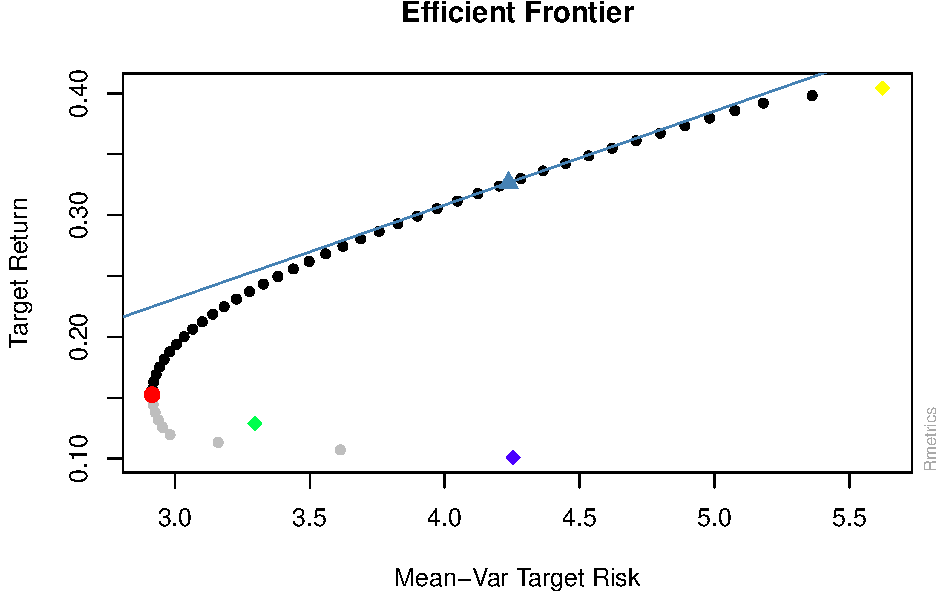
\includegraphics{Markowitz_Research_Me_files/figure-latex/unnamed-chunk-20-1.pdf}

\begin{Shaded}
\begin{Highlighting}[]
\KeywordTok{plot}\NormalTok{(effFrontier,}\KeywordTok{c}\NormalTok{(}\DecValTok{1}\NormalTok{,}\DecValTok{2}\NormalTok{))}
\end{Highlighting}
\end{Shaded}

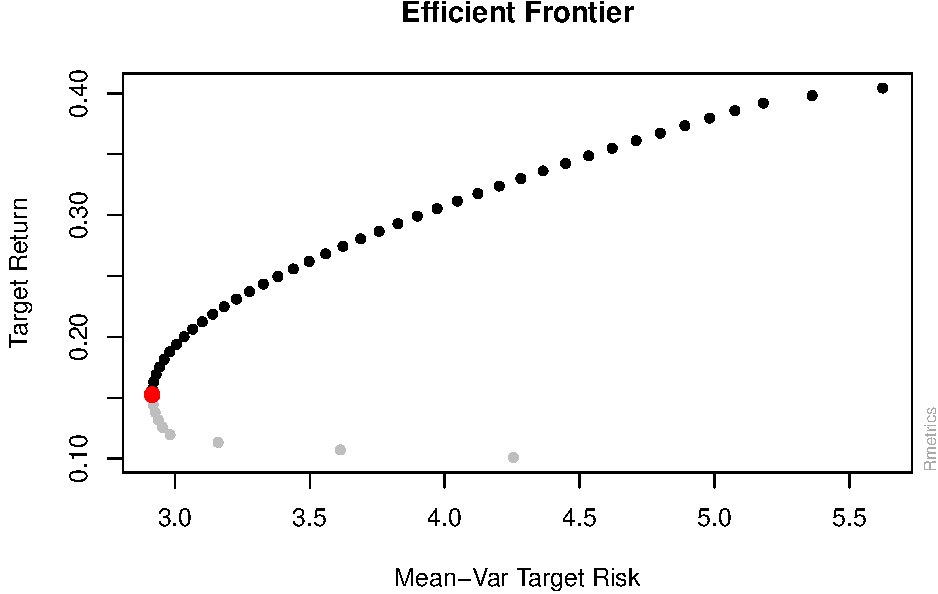
\includegraphics{Markowitz_Research_Me_files/figure-latex/unnamed-chunk-20-2.pdf}

\begin{Shaded}
\begin{Highlighting}[]
\KeywordTok{plot}\NormalTok{(effFrontier,}\KeywordTok{c}\NormalTok{(}\DecValTok{1}\NormalTok{,}\DecValTok{8}\NormalTok{))}
\end{Highlighting}
\end{Shaded}

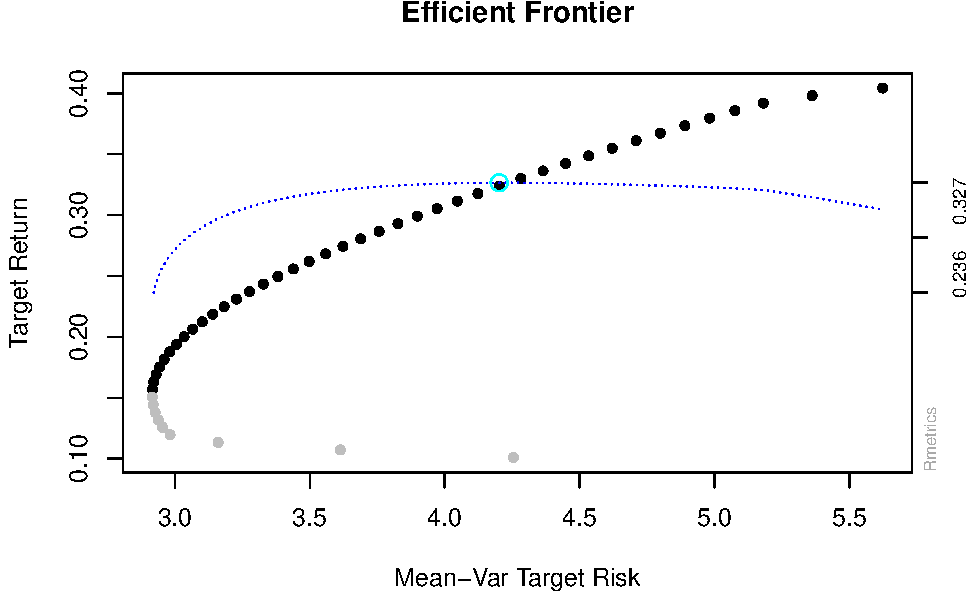
\includegraphics{Markowitz_Research_Me_files/figure-latex/unnamed-chunk-20-3.pdf}

\begin{Shaded}
\begin{Highlighting}[]
\CommentTok{#Plot Frontier Weights (Can Adjust Number of Points)}
\CommentTok{#get allocations for each instrument for each point on the efficient frontier}
\NormalTok{frontierWeights <-}\StringTok{ }\KeywordTok{getWeights}\NormalTok{(effFrontier) }
\KeywordTok{colnames}\NormalTok{(frontierWeights) <-}\StringTok{ }\NormalTok{tickers}
\NormalTok{risk_return <-}\StringTok{ }\KeywordTok{frontierPoints}\NormalTok{(effFrontier)}
\KeywordTok{write.csv}\NormalTok{(risk_return, }\StringTok{"risk_return.csv"}\NormalTok{)}

\CommentTok{#Output Correlation}
\NormalTok{cor_matrix <-}\StringTok{ }\KeywordTok{cor}\NormalTok{(portfolioReturns)}
\NormalTok{cov_matrix <-}\StringTok{ }\KeywordTok{cov}\NormalTok{(portfolioReturns)}
\KeywordTok{write.csv}\NormalTok{(cov_matrix, }\StringTok{"covmatrix.csv"}\NormalTok{)}
\NormalTok{cov_matrix}
\end{Highlighting}
\end{Shaded}

\begin{verbatim}
##            DIS      BABA       JNJ        FB
## DIS  18.096436  5.647140  4.629781  6.640169
## BABA  5.647140 50.863675  5.113207 13.648713
## JNJ   4.629781  5.113207 10.864806  6.147258
## FB    6.640169 13.648713  6.147258 31.617699
\end{verbatim}

\begin{Shaded}
\begin{Highlighting}[]
\CommentTok{#Annualize Data}
\CommentTok{#get risk and return values for points on the efficient frontier}
\NormalTok{riskReturnPoints <-}\StringTok{ }\KeywordTok{frontierPoints}\NormalTok{(effFrontier) }
\NormalTok{annualizedPoints <-}\StringTok{ }\KeywordTok{data.frame}\NormalTok{(}\DataTypeTok{targetRisk=}\NormalTok{riskReturnPoints[, }\StringTok{"targetRisk"}\NormalTok{]}\OperatorTok{*}\KeywordTok{sqrt}\NormalTok{(}\DecValTok{365}\NormalTok{),}
                               \DataTypeTok{targetReturn=}\NormalTok{riskReturnPoints[,}\StringTok{"targetReturn"}\NormalTok{]}\OperatorTok{*}\DecValTok{365}\NormalTok{)}
\KeywordTok{plot}\NormalTok{(annualizedPoints)}
\end{Highlighting}
\end{Shaded}

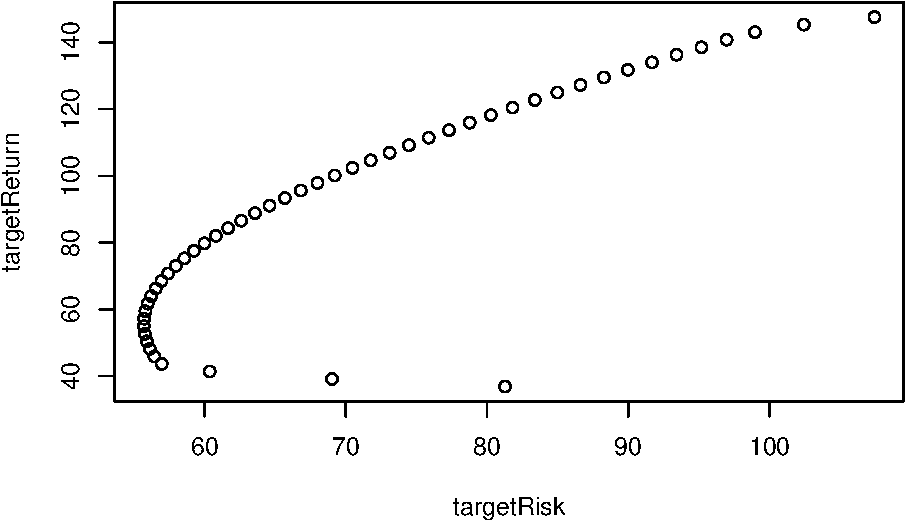
\includegraphics{Markowitz_Research_Me_files/figure-latex/unnamed-chunk-20-4.pdf}

\begin{Shaded}
\begin{Highlighting}[]
\CommentTok{# plot Sharpe ratios for each point on the efficient frontier}
\NormalTok{riskFreeRate <-}\StringTok{ }\DecValTok{0}
\KeywordTok{plot}\NormalTok{((annualizedPoints[,}\StringTok{"targetReturn"}\NormalTok{]}\OperatorTok{-}\NormalTok{riskFreeRate) }\OperatorTok{/}\StringTok{ }\NormalTok{annualizedPoints[,}\StringTok{"targetRisk"}\NormalTok{],}
     \DataTypeTok{xlab=}\StringTok{"point on efficient frontier"}\NormalTok{, }\DataTypeTok{ylab=}\StringTok{"Sharpe ratio"}\NormalTok{)}
\end{Highlighting}
\end{Shaded}

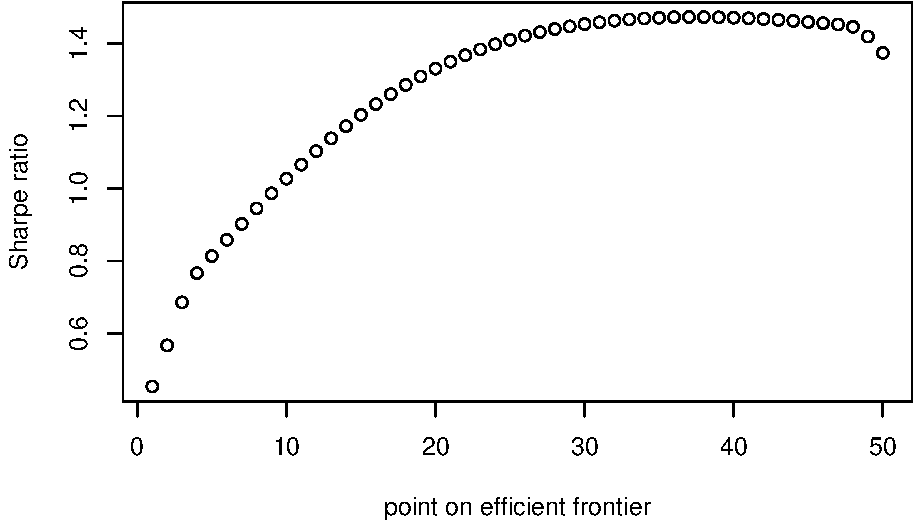
\includegraphics{Markowitz_Research_Me_files/figure-latex/unnamed-chunk-20-5.pdf}

\begin{Shaded}
\begin{Highlighting}[]
\CommentTok{#Plot Frontier Weights (Need to transpose matrix first)}
\KeywordTok{barplot}\NormalTok{(}\KeywordTok{t}\NormalTok{(frontierWeights), }\DataTypeTok{main=}\StringTok{"Frontier Weights"}\NormalTok{, }
        \DataTypeTok{col=}\KeywordTok{cm.colors}\NormalTok{(}\KeywordTok{ncol}\NormalTok{(frontierWeights)}\OperatorTok{+}\DecValTok{2}\NormalTok{), }
        \DataTypeTok{legend=}\KeywordTok{colnames}\NormalTok{(frontierWeights))}
\end{Highlighting}
\end{Shaded}

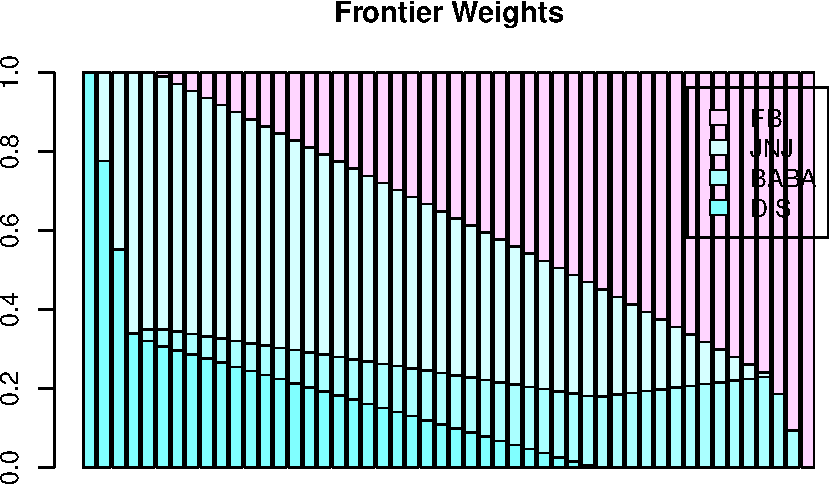
\includegraphics{Markowitz_Research_Me_files/figure-latex/unnamed-chunk-20-6.pdf}

\begin{Shaded}
\begin{Highlighting}[]
\CommentTok{#Get Minimum Variance Port, Tangency Port, etc.}
\CommentTok{#mvp = minimum variance portfolio}
\NormalTok{mvp <-}\StringTok{ }\KeywordTok{minvariancePortfolio}\NormalTok{(portfolioReturns,}
                            \DataTypeTok{spec=}\KeywordTok{portfolioSpec}\NormalTok{(), }\DataTypeTok{constraints=}\StringTok{"LongOnly"}\NormalTok{)}
\NormalTok{mvp}
\end{Highlighting}
\end{Shaded}

\begin{verbatim}
## 
## Title:
##  MV Minimum Variance Portfolio 
##  Estimator:         covEstimator 
##  Solver:            solveRquadprog 
##  Optimize:          minRisk 
##  Constraints:       LongOnly 
## 
## Portfolio Weights:
##    DIS   BABA    JNJ     FB 
## 0.2727 0.0578 0.5994 0.0701 
## 
## Covariance Risk Budgets:
##    DIS   BABA    JNJ     FB 
## 0.2727 0.0578 0.5994 0.0701 
## 
## Target Returns and Risks:
##   mean    Cov   CVaR    VaR 
## 0.1526 2.9157 6.7967 4.8266 
## 
## Description:
##  Mon Jan  7 18:21:42 2019 by user: kirui
\end{verbatim}

\begin{Shaded}
\begin{Highlighting}[]
\NormalTok{tangencyPort <-}\StringTok{ }\KeywordTok{tangencyPortfolio}\NormalTok{(portfolioReturns,}
                                  \DataTypeTok{spec=}\KeywordTok{portfolioSpec}\NormalTok{(),}\DataTypeTok{constraints=}\StringTok{"LongOnly"}\NormalTok{)}
\NormalTok{tangencyPort}
\end{Highlighting}
\end{Shaded}

\begin{verbatim}
## 
## Title:
##  MV Tangency Portfolio 
##  Estimator:         covEstimator 
##  Solver:            solveRquadprog 
##  Optimize:          minRisk 
##  Constraints:       LongOnly 
## 
## Portfolio Weights:
##    DIS   BABA    JNJ     FB 
## 0.0000 0.1868 0.2372 0.5760 
## 
## Covariance Risk Budgets:
##    DIS   BABA    JNJ     FB 
## 0.0000 0.1933 0.0935 0.7132 
## 
## Target Returns and Risks:
##   mean    Cov   CVaR    VaR 
## 0.3265 4.2364 9.8855 6.3517 
## 
## Description:
##  Mon Jan  7 18:21:42 2019 by user: kirui
\end{verbatim}

\begin{Shaded}
\begin{Highlighting}[]
\NormalTok{mvpweights <-}\StringTok{ }\KeywordTok{getWeights}\NormalTok{(mvp) }\CommentTok{#mininum variance portfolio weights}
\NormalTok{tangencyweights <-}\StringTok{ }\KeywordTok{getWeights}\NormalTok{(tangencyPort) }\CommentTok{#tangency portfolio weights}
\CommentTok{#ggplot of MVP Weights}
\NormalTok{df <-}\StringTok{ }\KeywordTok{data.frame}\NormalTok{(mvpweights)}
\NormalTok{assets <-}\StringTok{ }\KeywordTok{colnames}\NormalTok{(frontierWeights)}
\KeywordTok{ggplot}\NormalTok{(}\DataTypeTok{data=}\NormalTok{df, }\KeywordTok{aes}\NormalTok{(}\DataTypeTok{x=}\NormalTok{assets, }\DataTypeTok{y=}\NormalTok{mvpweights, }\DataTypeTok{fill=}\NormalTok{assets)) }\OperatorTok{+}
\StringTok{  }\KeywordTok{geom_bar}\NormalTok{(}\DataTypeTok{stat=}\StringTok{"identity"}\NormalTok{, }\DataTypeTok{position=}\KeywordTok{position_dodge}\NormalTok{(),}\DataTypeTok{colour=}\StringTok{"black"}\NormalTok{) }\OperatorTok{+}
\StringTok{  }\KeywordTok{geom_text}\NormalTok{(}\KeywordTok{aes}\NormalTok{(}\DataTypeTok{label=}\KeywordTok{sprintf}\NormalTok{(}\StringTok{"%.02f %%"}\NormalTok{,mvpweights}\OperatorTok{*}\DecValTok{100}\NormalTok{)),}
            \DataTypeTok{position=}\KeywordTok{position_dodge}\NormalTok{(}\DataTypeTok{width=}\FloatTok{0.9}\NormalTok{), }\DataTypeTok{vjust=}\OperatorTok{-}\FloatTok{0.25}\NormalTok{, }\DataTypeTok{check_overlap =} \OtherTok{TRUE}\NormalTok{) }\OperatorTok{+}
\StringTok{              }\KeywordTok{ggtitle}\NormalTok{(}\StringTok{"Minimum Variance Portfolio Optimal Weights"}\NormalTok{)}\OperatorTok{+}
\StringTok{  }\KeywordTok{theme}\NormalTok{(}\DataTypeTok{plot.title =} \KeywordTok{element_text}\NormalTok{(}\DataTypeTok{hjust =} \FloatTok{0.5}\NormalTok{)) }\OperatorTok{+}
\StringTok{  }\KeywordTok{labs}\NormalTok{(}\DataTypeTok{x=} \StringTok{"Assets"}\NormalTok{, }\DataTypeTok{y =} \StringTok{"Weights (%)"}\NormalTok{)}
\end{Highlighting}
\end{Shaded}

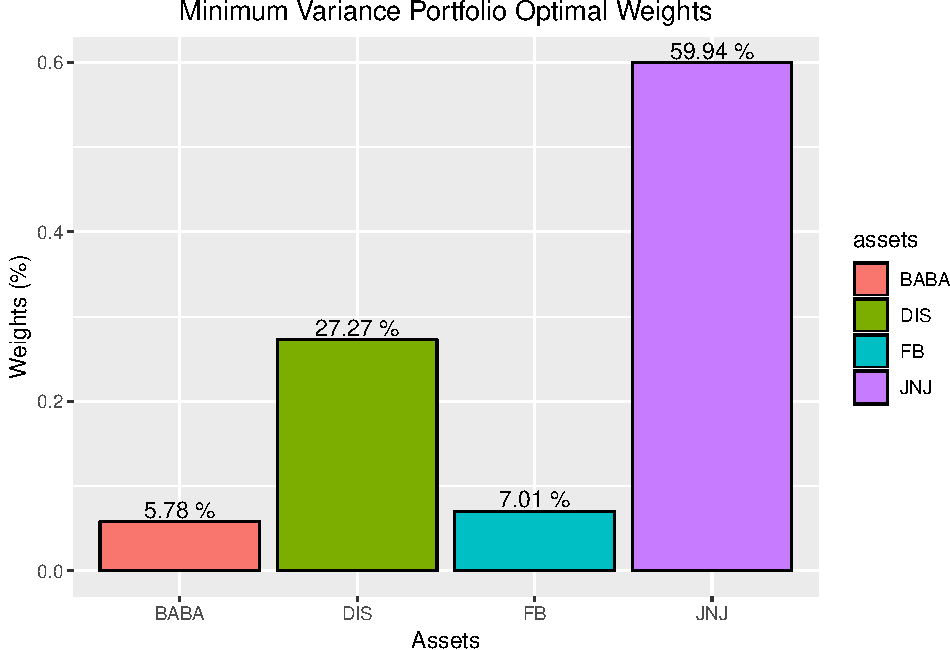
\includegraphics{Markowitz_Research_Me_files/figure-latex/unnamed-chunk-20-7.pdf}

\begin{Shaded}
\begin{Highlighting}[]
\CommentTok{#ggplot of tangency portfolio weights }
\NormalTok{dft <-}\StringTok{ }\KeywordTok{data.frame}\NormalTok{(tangencyweights)}
\NormalTok{assets <-}\StringTok{ }\KeywordTok{colnames}\NormalTok{(frontierWeights)}
\KeywordTok{ggplot}\NormalTok{(}\DataTypeTok{data=}\NormalTok{dft, }\KeywordTok{aes}\NormalTok{(}\DataTypeTok{x=}\NormalTok{assets, }\DataTypeTok{y=}\NormalTok{tangencyweights, }\DataTypeTok{fill=}\NormalTok{assets)) }\OperatorTok{+}
\StringTok{  }\KeywordTok{geom_bar}\NormalTok{(}\DataTypeTok{stat=}\StringTok{"identity"}\NormalTok{, }\DataTypeTok{position=}\KeywordTok{position_dodge}\NormalTok{(),}\DataTypeTok{colour=}\StringTok{"black"}\NormalTok{) }\OperatorTok{+}
\StringTok{  }\KeywordTok{geom_text}\NormalTok{(}\KeywordTok{aes}\NormalTok{(}\DataTypeTok{label=}\KeywordTok{sprintf}\NormalTok{(}\StringTok{"%.02f %%"}\NormalTok{,tangencyweights}\OperatorTok{*}\DecValTok{100}\NormalTok{)),}
            \DataTypeTok{position=}\KeywordTok{position_dodge}\NormalTok{(}\DataTypeTok{width=}\FloatTok{0.9}\NormalTok{), }\DataTypeTok{vjust=}\OperatorTok{-}\FloatTok{0.25}\NormalTok{, }\DataTypeTok{check_overlap =} \OtherTok{TRUE}\NormalTok{) }\OperatorTok{+}
\StringTok{  }\KeywordTok{ggtitle}\NormalTok{(}\StringTok{"Tangency Portfolio Weights"}\NormalTok{)}\OperatorTok{+}\StringTok{ }\KeywordTok{theme}\NormalTok{(}\DataTypeTok{plot.title =} \KeywordTok{element_text}\NormalTok{(}\DataTypeTok{hjust =} \FloatTok{0.5}\NormalTok{)) }\OperatorTok{+}
\StringTok{  }\KeywordTok{labs}\NormalTok{(}\DataTypeTok{x=} \StringTok{"Assets"}\NormalTok{, }\DataTypeTok{y =} \StringTok{"Weights (%)"}\NormalTok{)}
\end{Highlighting}
\end{Shaded}

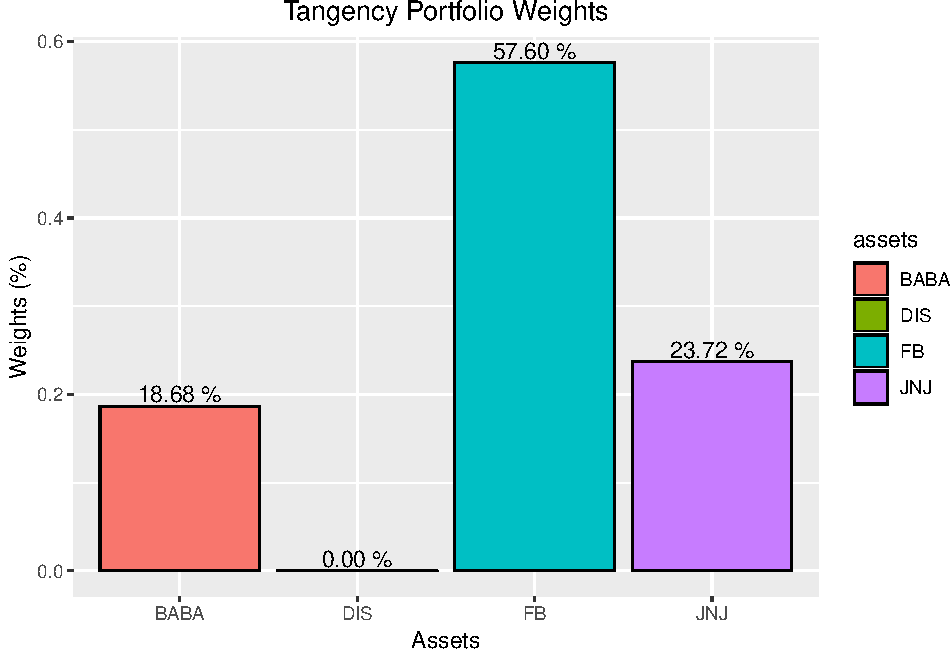
\includegraphics{Markowitz_Research_Me_files/figure-latex/unnamed-chunk-20-8.pdf}

\subsubsection{Note:}\label{note}

\begin{itemize}
\item
  The function \textbf{portfolioFrontier} calculates the whole efficient
  frontier. The portfolio information consists of five arguments: data,
  specifications, constraints, title and description. Tha range of the
  frontier is determined from the range of asset returns, and the number
  of equidistant points in the returns, is calculated from the number of
  frontier points hold in the specification structure.
\item
  An efficient portfolio ia a portfolio which lies on the efficient
  frontier. The \textbf{efficientPortfolio} function returns the
  properties of the efficient portfolio.
\item
  The function \textbf{tangencyPortfolio} returns the portfolio with the
  highest return/risk ratio on the efficient frontier. For the
  Markowitz, this is the same as the Share Ratio. To find this point on
  the frontier thr return/risk ratio calculated from the target return
  and target risk returned by the function \textbf{efficientPortfolio}.
\item
  The function \textbf{minvariancePortfolio} returns the portfolio with
  the minimal risk on the efficient frontier. To find the minimal risk
  point, the target risk returned by the function
  \textbf{efficientPortfolio} is minimized.
\item
  The function \textbf{maxreturnPortfolio} returns the portfolio with
  the maximal return for a fixed target risk.
\end{itemize}

You will realize that we have multiplied the daily returns by 252 and
multiplied the deviation by square root of 252. The reason is that the
Sharpe Ratio is typically defined in terms of annual return and annual
deviation. As everyone has said, you go from daily returns to annual
returns by assuming daily returns are independent and identically
distributed.

With that assumption, you get annual return by multiplying by daily
return by 252 (compounding makes little difference when daily return is
1 ). You get annual deviation by multiplying daily deviation by square
root of 252

\subsection{Examining the portfolio with
constraints}\label{examining-the-portfolio-with-constraints}

\subsubsection{Portfolio with Short selling
allowed}\label{portfolio-with-short-selling-allowed}

We will now examine the portfolio having some constraints and
specifications. We will alow shortselling in this portfolio and set the
minimum and maximimum weight in one given asset throughout the entire
list of tickers.

\begin{Shaded}
\begin{Highlighting}[]
\CommentTok{#Set Specs}
\NormalTok{Spec =}\StringTok{ }\KeywordTok{portfolioSpec}\NormalTok{()}
\KeywordTok{setSolver}\NormalTok{(Spec) =}\StringTok{ "solveRshortExact"} \CommentTok{#set the solver to use}
\KeywordTok{setTargetRisk}\NormalTok{(Spec) =}\StringTok{ }\NormalTok{.}\DecValTok{12} \CommentTok{#set the target risk level.}
\NormalTok{constraints <-}\StringTok{ }\KeywordTok{c}\NormalTok{(}\StringTok{"minW[1:length(tickers)]=-1"}\NormalTok{,}\StringTok{"maxW[1:length(tickers)]=.60"}\NormalTok{, }\StringTok{"Short"}\NormalTok{)}
 
\NormalTok{effFrontierShort <-}\StringTok{ }\KeywordTok{portfolioFrontier}\NormalTok{(portfolioReturns, Spec, }\DataTypeTok{constraints =}\NormalTok{ constraints)}
\end{Highlighting}
\end{Shaded}

\begin{verbatim}
## Warning in as.vector(invSigma %*% one)/(one %*% invSigma %*% one): Recycling array of length 1 in vector-array arithmetic is deprecated.
##   Use c() or as.vector() instead.
\end{verbatim}

\begin{Shaded}
\begin{Highlighting}[]
\NormalTok{weights <-}\StringTok{ }\KeywordTok{getWeights}\NormalTok{(effFrontierShort)}
\KeywordTok{write.csv}\NormalTok{(weights, }\StringTok{"weightsShort.csv"}\NormalTok{)}
\KeywordTok{colnames}\NormalTok{(weights) <-}\StringTok{ }\NormalTok{tickers}
\CommentTok{#Plot the efficient frontier with minimun variance portfolio and tangency portfolio.}
\KeywordTok{plot}\NormalTok{(effFrontierShort, }\KeywordTok{c}\NormalTok{(}\DecValTok{1}\NormalTok{, }\DecValTok{2}\NormalTok{, }\DecValTok{3}\NormalTok{,}\DecValTok{4}\NormalTok{))}
\end{Highlighting}
\end{Shaded}

\begin{verbatim}
## Warning in as.vector(invSigma %*% one)/(one %*% invSigma %*% one): Recycling array of length 1 in vector-array arithmetic is deprecated.
##   Use c() or as.vector() instead.
\end{verbatim}

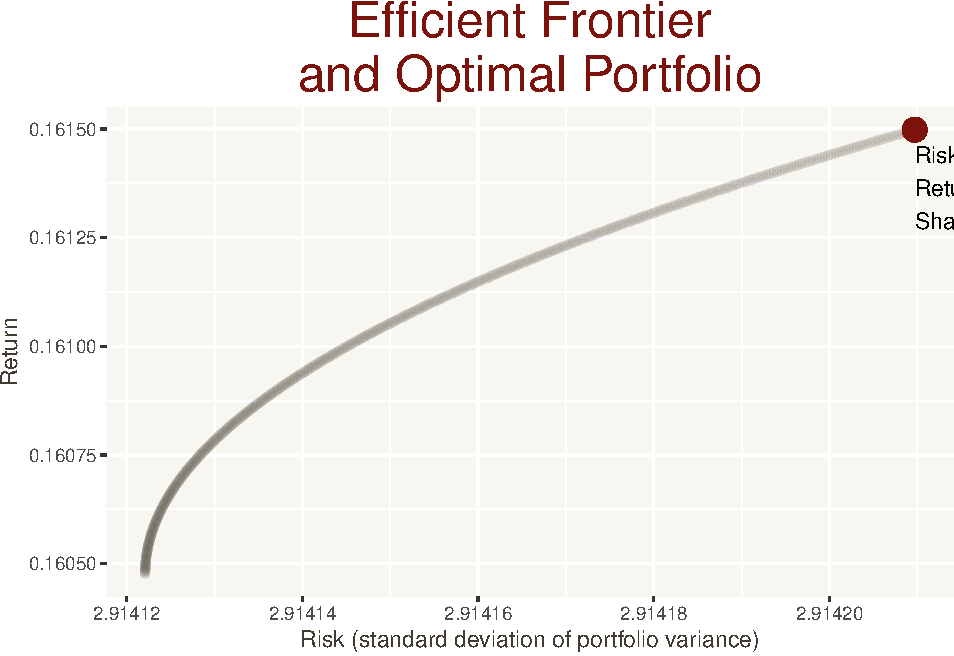
\includegraphics{Markowitz_Research_Me_files/figure-latex/unnamed-chunk-21-1.pdf}

\begin{Shaded}
\begin{Highlighting}[]
\CommentTok{#Plot Frontier Weights (Need to transpose matrix first)}
\KeywordTok{barplot}\NormalTok{(}\KeywordTok{t}\NormalTok{(weights), }\DataTypeTok{main=}\StringTok{"Frontier Weights"}\NormalTok{, }
        \DataTypeTok{col=}\KeywordTok{cm.colors}\NormalTok{(}\KeywordTok{ncol}\NormalTok{(weights)}\OperatorTok{+}\DecValTok{2}\NormalTok{), }\DataTypeTok{legend=}\KeywordTok{colnames}\NormalTok{(weights))}
\end{Highlighting}
\end{Shaded}

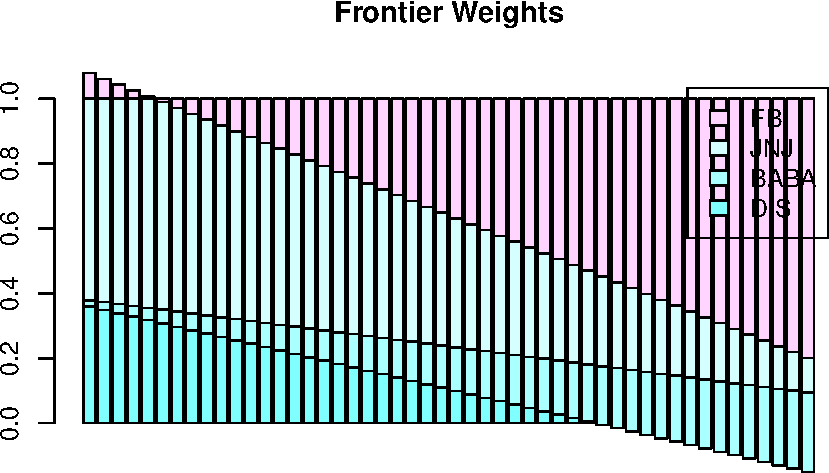
\includegraphics{Markowitz_Research_Me_files/figure-latex/unnamed-chunk-21-2.pdf}

\begin{Shaded}
\begin{Highlighting}[]
\NormalTok{effPortShort <-}\StringTok{ }\KeywordTok{minvariancePortfolio}\NormalTok{(portfolioReturns, Spec, }\DataTypeTok{constraints=}\NormalTok{constraints)}
\end{Highlighting}
\end{Shaded}

\begin{verbatim}
## Warning in as.vector(invSigma %*% one)/(one %*% invSigma %*% one): Recycling array of length 1 in vector-array arithmetic is deprecated.
##   Use c() or as.vector() instead.
\end{verbatim}

\begin{Shaded}
\begin{Highlighting}[]
\NormalTok{optWeights <-}\StringTok{ }\KeywordTok{getWeights}\NormalTok{(effPortShort)}
\NormalTok{tanPortShort <-}\StringTok{ }\KeywordTok{tangencyPortfolio}\NormalTok{(portfolioReturns, Spec, }\DataTypeTok{constraints=}\NormalTok{constraints)}
\NormalTok{tanWeights <-}\StringTok{ }\KeywordTok{getWeights}\NormalTok{(tanPortShort)}
\CommentTok{#maxR <- maxreturnPortfolio(portfolioReturns , Spec, constraints=constraints)}
\CommentTok{#maxWeights <- getWeights(maxR)}
 
\CommentTok{#ggplot MVP Weights}
\NormalTok{df <-}\StringTok{ }\KeywordTok{data.frame}\NormalTok{(tanWeights)}
\NormalTok{assets <-}\StringTok{ }\KeywordTok{colnames}\NormalTok{(frontierWeights)}
\KeywordTok{ggplot}\NormalTok{(}\DataTypeTok{data=}\NormalTok{df, }\KeywordTok{aes}\NormalTok{(}\DataTypeTok{x=}\NormalTok{assets, }\DataTypeTok{y=}\NormalTok{tanWeights, }\DataTypeTok{fill=}\NormalTok{assets)) }\OperatorTok{+}
\StringTok{  }\KeywordTok{geom_bar}\NormalTok{(}\DataTypeTok{stat=}\StringTok{"identity"}\NormalTok{, }\DataTypeTok{position=}\KeywordTok{position_dodge}\NormalTok{(),}\DataTypeTok{colour=}\StringTok{"black"}\NormalTok{) }\OperatorTok{+}
\StringTok{  }\KeywordTok{geom_text}\NormalTok{(}\KeywordTok{aes}\NormalTok{(}\DataTypeTok{label=}\KeywordTok{sprintf}\NormalTok{(}\StringTok{"%.02f %%"}\NormalTok{,tanWeights}\OperatorTok{*}\DecValTok{100}\NormalTok{)),}
            \DataTypeTok{position=}\KeywordTok{position_dodge}\NormalTok{(}\DataTypeTok{width=}\FloatTok{0.9}\NormalTok{), }\DataTypeTok{vjust=}\OperatorTok{-}\FloatTok{0.25}\NormalTok{, }\DataTypeTok{check_overlap =} \OtherTok{TRUE}\NormalTok{) }\OperatorTok{+}
\StringTok{  }\KeywordTok{ggtitle}\NormalTok{(}\StringTok{"Tangency Portfolio With Shorts Allowed"}\NormalTok{)}\OperatorTok{+}\StringTok{ }
\StringTok{  }\KeywordTok{theme}\NormalTok{(}\DataTypeTok{plot.title =} \KeywordTok{element_text}\NormalTok{(}\DataTypeTok{hjust =} \FloatTok{0.5}\NormalTok{)) }\OperatorTok{+}
\StringTok{  }\KeywordTok{labs}\NormalTok{(}\DataTypeTok{x=} \StringTok{"Assets"}\NormalTok{, }\DataTypeTok{y =} \StringTok{"Weight (%)"}\NormalTok{)}
\end{Highlighting}
\end{Shaded}

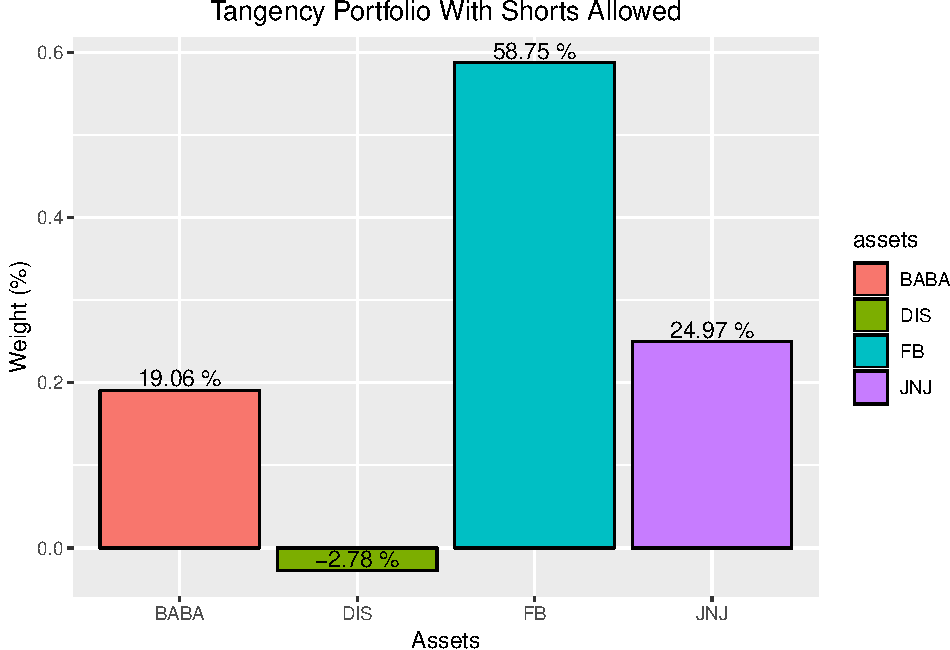
\includegraphics{Markowitz_Research_Me_files/figure-latex/unnamed-chunk-21-3.pdf}

\subsection{Markowitz model with a risk free
asset}\label{markowitz-model-with-a-risk-free-asset}

\subsubsection{function to create asset
allocation}\label{function-to-create-asset-allocation}

\begin{Shaded}
\begin{Highlighting}[]
\NormalTok{graph.asset.allocation =}\StringTok{ }\ControlFlowTok{function}\NormalTok{(portfolio,sd,mu, }\DataTypeTok{png.name=}\StringTok{"optimal-asset-allocation-mu.png"}\NormalTok{,}\DataTypeTok{title=}\StringTok{"Markowitz: asset allocation"}\NormalTok{)\{}
\NormalTok{  nr =}\StringTok{ }\KeywordTok{dim}\NormalTok{(portfolio)[}\DecValTok{1}\NormalTok{]}
\NormalTok{  titles =}\StringTok{ }\KeywordTok{row.names}\NormalTok{(portfolio)}
  \CommentTok{#print(portfolio)}
  \CommentTok{#print(titles)}

  \KeywordTok{par}\NormalTok{(}\DataTypeTok{mar=}\KeywordTok{c}\NormalTok{(}\DecValTok{5}\NormalTok{,}\DecValTok{4}\NormalTok{,}\DecValTok{4}\NormalTok{,}\DecValTok{5}\NormalTok{)}\OperatorTok{+}\NormalTok{.}\DecValTok{1}\NormalTok{)}
  \KeywordTok{plot}\NormalTok{(mu,}\KeywordTok{t}\NormalTok{(portfolio[}\DecValTok{1}\NormalTok{,]),}\DataTypeTok{ylim=}\KeywordTok{c}\NormalTok{(}\KeywordTok{min}\NormalTok{(portfolio),}\KeywordTok{max}\NormalTok{(portfolio)),}\DataTypeTok{type=}\StringTok{'l'}\NormalTok{,}\DataTypeTok{col=}\DecValTok{1}\NormalTok{,}\DataTypeTok{lty=}\DecValTok{1}\NormalTok{,}\DataTypeTok{ylab=}\StringTok{"x* asset allocation"}\NormalTok{)}
  \ControlFlowTok{for}\NormalTok{ (j }\ControlFlowTok{in} \DecValTok{2}\OperatorTok{:}\NormalTok{nr) }\KeywordTok{lines}\NormalTok{(mu,}\KeywordTok{t}\NormalTok{(portfolio[j,]),}\DataTypeTok{type=}\StringTok{'l'}\NormalTok{,}\DataTypeTok{col=}\NormalTok{j,}\DataTypeTok{lty=}\NormalTok{j)}
  \KeywordTok{par}\NormalTok{(}\DataTypeTok{new=}\OtherTok{TRUE}\NormalTok{)}
  \KeywordTok{plot}\NormalTok{(mu, sd,}\DataTypeTok{type=}\StringTok{"l"}\NormalTok{,}\DataTypeTok{col=}\StringTok{"darkgray"}\NormalTok{,}\DataTypeTok{lwd=}\DecValTok{3}\NormalTok{,}\DataTypeTok{lty=}\DecValTok{6}\NormalTok{,}\DataTypeTok{xaxt=}\StringTok{"n"}\NormalTok{,}\DataTypeTok{yaxt=}\StringTok{"n"}\NormalTok{,}\DataTypeTok{xlab=}\StringTok{""}\NormalTok{,}\DataTypeTok{ylab=}\StringTok{""}\NormalTok{)}
  \KeywordTok{axis}\NormalTok{(}\DecValTok{4}\NormalTok{)}
  \KeywordTok{mtext}\NormalTok{(}\StringTok{"sd(x*(mu))"}\NormalTok{,}\DataTypeTok{side=}\DecValTok{4}\NormalTok{,}\DataTypeTok{line=}\DecValTok{3}\NormalTok{,}\DataTypeTok{col=}\StringTok{"darkgray"}\NormalTok{)}
  \KeywordTok{legend}\NormalTok{(}\StringTok{"topleft"}\NormalTok{, }\KeywordTok{c}\NormalTok{(titles), }\DataTypeTok{col=}\KeywordTok{c}\NormalTok{(}\DecValTok{1}\OperatorTok{:}\NormalTok{nr), }\DataTypeTok{lty=}\DecValTok{1}\OperatorTok{:}\NormalTok{nr,}\DataTypeTok{bty=}\StringTok{"n"}\NormalTok{,}\DataTypeTok{lwd=}\KeywordTok{rep}\NormalTok{(}\DecValTok{1}\NormalTok{,nr)) }
\NormalTok{\}}
\end{Highlighting}
\end{Shaded}

\begin{Shaded}
\begin{Highlighting}[]
\NormalTok{markowitz.portfolio.cash =}\StringTok{ }\ControlFlowTok{function}\NormalTok{(mu.ret, }\DataTypeTok{Cov.Matrix=}\KeywordTok{diag}\NormalTok{(}\KeywordTok{length}\NormalTok{(mu.ret)), }\DataTypeTok{mu.portfolio.min =} \DecValTok{0}\NormalTok{, }\DataTypeTok{r0=}\DecValTok{0}\NormalTok{)\{}
  \ControlFlowTok{if}\NormalTok{ (}\KeywordTok{missing}\NormalTok{(mu.ret)) }\KeywordTok{stop}\NormalTok{(}\StringTok{"need vector of expected asset returns: mu.ret"}\NormalTok{)}
\NormalTok{  titles=}\StringTok{ }\KeywordTok{names}\NormalTok{(mu.ret)}
  
\NormalTok{  nr =}\StringTok{ }\KeywordTok{length}\NormalTok{(mu.ret)}
  \ControlFlowTok{if}\NormalTok{ (}\KeywordTok{sum}\NormalTok{(}\KeywordTok{dim}\NormalTok{(Cov.Matrix)}\OperatorTok{==}\NormalTok{nr)}\OperatorTok{<}\DecValTok{2}\NormalTok{) }\KeywordTok{stop}\NormalTok{(}\StringTok{"wrong dimensions"}\NormalTok{)}
\NormalTok{  ones =}\StringTok{ }\KeywordTok{rep}\NormalTok{(}\DecValTok{1}\NormalTok{,nr)}
\NormalTok{  Cov.inv =}\StringTok{ }\KeywordTok{solve}\NormalTok{(Cov.Matrix)}
  
\NormalTok{  m =}\StringTok{ }\KeywordTok{length}\NormalTok{(mu.portfolio.min)}
\NormalTok{  xm.r0 =}\StringTok{ }\KeywordTok{matrix}\NormalTok{(}\DataTypeTok{nrow =}\NormalTok{ nr}\OperatorTok{+}\DecValTok{1}\NormalTok{, }\DataTypeTok{ncol=}\NormalTok{m)}
  \CommentTok{#first nr compontens usual assets x^star, nr+1 = cash(r0) x0^star}
  
\NormalTok{  a =}\StringTok{ }\KeywordTok{as.numeric}\NormalTok{(mu.ret}\OperatorTok\StringTok{ }\NormalTok{Cov.inv }\OperatorTok\StringTok{ }\NormalTok{mu.ret)}
\NormalTok{  b =}\StringTok{ }\KeywordTok{as.numeric}\NormalTok{(mu.ret}\OperatorTok\StringTok{ }\NormalTok{Cov.inv }\OperatorTok\StringTok{ }\NormalTok{ones )}
\NormalTok{  c =}\StringTok{ }\KeywordTok{as.numeric}\NormalTok{(ones }\OperatorTok\StringTok{ }\NormalTok{Cov.inv }\OperatorTok\StringTok{ }\NormalTok{ones )}
\NormalTok{  d =}\StringTok{ }\NormalTok{a}\OperatorTok{-}\DecValTok{2}\OperatorTok{*}\NormalTok{b}\OperatorTok{*}\NormalTok{r0}\OperatorTok{+}\NormalTok{c}\OperatorTok{*}\NormalTok{r0}\OperatorTok{*}\NormalTok{r0}
  
  \ControlFlowTok{for}\NormalTok{ (k }\ControlFlowTok{in} \DecValTok{1}\OperatorTok{:}\NormalTok{m)\{}
\NormalTok{    xm.r0[,k] =}\StringTok{ }\KeywordTok{c}\NormalTok{((mu.portfolio.min[k]}\OperatorTok{-}\NormalTok{r0)}\OperatorTok{*}\NormalTok{(Cov.inv}\OperatorTok\NormalTok{mu.ret }\OperatorTok{-}\StringTok{ }\NormalTok{r0 }\OperatorTok{*}\StringTok{ }\NormalTok{Cov.inv}\OperatorTok\NormalTok{ones),d}\OperatorTok{-}\NormalTok{(b}\OperatorTok{-}\NormalTok{r0}\OperatorTok{*}\NormalTok{c)}\OperatorTok{*}\NormalTok{(mu.portfolio.min[k]}\OperatorTok{-}\NormalTok{r0)) }
\NormalTok{  \}}
  
  \ControlFlowTok{if}\NormalTok{ (}\KeywordTok{length}\NormalTok{(titles)}\OperatorTok{==}\DecValTok{0}\NormalTok{) titles=}\KeywordTok{paste}\NormalTok{(}\KeywordTok{rep}\NormalTok{(}\StringTok{"asset"}\NormalTok{,nr),}\DecValTok{1}\OperatorTok{:}\NormalTok{nr)}
  \KeywordTok{print}\NormalTok{(titles)}
  \KeywordTok{row.names}\NormalTok{(xm.r0) =}\StringTok{ }\KeywordTok{c}\NormalTok{(titles,}\StringTok{"cash"}\NormalTok{)}
\NormalTok{  standarddev =}\StringTok{ }\KeywordTok{sqrt}\NormalTok{(((mu.portfolio.min}\OperatorTok{-}\NormalTok{r0)}\OperatorTok{^}\DecValTok{2}\OperatorTok{/}\NormalTok{d))  }
\NormalTok{  return.list =}\StringTok{ }\KeywordTok{list}\NormalTok{(xm.r0}\OperatorTok{/}\NormalTok{d,standarddev)}
  \KeywordTok{names}\NormalTok{(return.list) =}\StringTok{ }\KeywordTok{c}\NormalTok{(}\StringTok{"efficient_portfolio"}\NormalTok{,}\StringTok{"standarddev"}\NormalTok{)}
  \KeywordTok{return}\NormalTok{(return.list)}
\NormalTok{\}}

\NormalTok{r0 =}\StringTok{ }\FloatTok{0.02}

\NormalTok{mu.new =}\StringTok{ }\KeywordTok{seq}\NormalTok{(}\DataTypeTok{from=}\FloatTok{0.0}\NormalTok{, }\DataTypeTok{by=}\FloatTok{0.01}\NormalTok{, }\DataTypeTok{to=}\FloatTok{0.84}\NormalTok{)}

\NormalTok{portfolio.riskfree =}\StringTok{ }\KeywordTok{markowitz.portfolio.cash}\NormalTok{(returns,Covar,mu.new,r0)}
\end{Highlighting}
\end{Shaded}

\begin{verbatim}
## [1] "DIS"  "BABA" "JNJ"  "FB"
\end{verbatim}

\begin{Shaded}
\begin{Highlighting}[]
\KeywordTok{colSums}\NormalTok{(portfolio.riskfree}\OperatorTok{$}\NormalTok{efficient_portfolio)}
\end{Highlighting}
\end{Shaded}

\begin{verbatim}
##  [1] 1 1 1 1 1 1 1 1 1 1 1 1 1 1 1 1 1 1 1 1 1 1 1 1 1 1 1 1 1 1 1 1 1 1 1
## [36] 1 1 1 1 1 1 1 1 1 1 1 1 1 1 1 1 1 1 1 1 1 1 1 1 1 1 1 1 1 1 1 1 1 1 1
## [71] 1 1 1 1 1 1 1 1 1 1 1 1 1 1 1
\end{verbatim}

\begin{Shaded}
\begin{Highlighting}[]
\KeywordTok{graph.asset.allocation}\NormalTok{(}\DataTypeTok{portfolio=}\NormalTok{portfolio.riskfree}\OperatorTok{$}\NormalTok{efficient_portfolio,}\DataTypeTok{sd=}\NormalTok{portfolio.riskfree}\OperatorTok{$}\NormalTok{standarddev, }
                       \DataTypeTok{mu=}\NormalTok{mu.new)}
\end{Highlighting}
\end{Shaded}

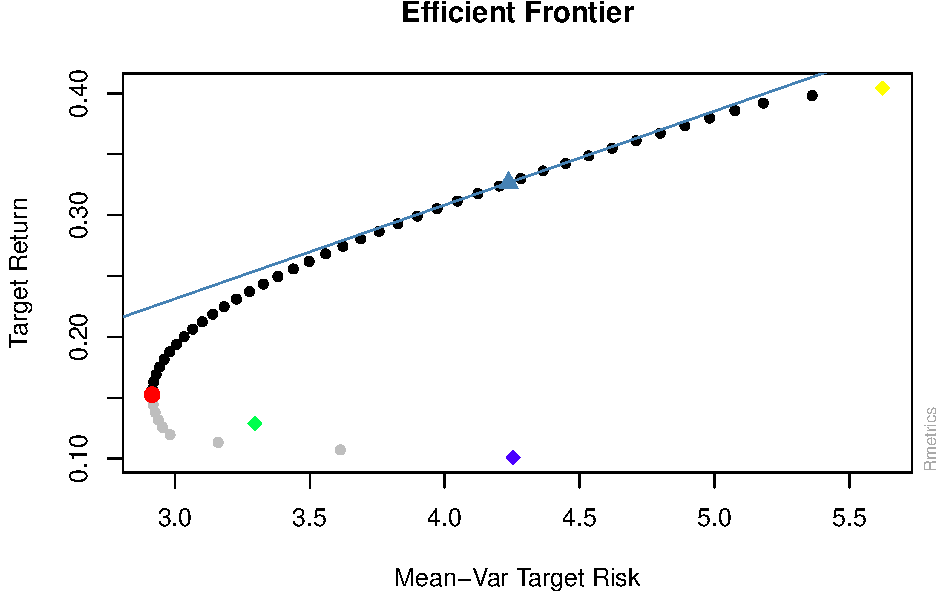
\includegraphics{Markowitz_Research_Me_files/figure-latex/unnamed-chunk-23-1.pdf}

\begin{Shaded}
\begin{Highlighting}[]
\CommentTok{# Using stacked barplot}
\NormalTok{asset_free <-}\StringTok{ }\KeywordTok{data.frame}\NormalTok{(mu.new,}\KeywordTok{t}\NormalTok{(portfolio.riskfree}\OperatorTok{$}\NormalTok{efficient_portfolio))}
\KeywordTok{library}\NormalTok{(reshape2)}
\NormalTok{asset_free <-}\StringTok{ }\KeywordTok{melt}\NormalTok{(asset_free, }\DataTypeTok{id =} \StringTok{"mu.new"}\NormalTok{)}
\KeywordTok{names}\NormalTok{(asset_free) <-}\StringTok{ }\KeywordTok{c}\NormalTok{(}\StringTok{"mu"}\NormalTok{,}\StringTok{"Stocks"}\NormalTok{,}\StringTok{"Allocation"}\NormalTok{)}
\KeywordTok{ggplot}\NormalTok{() }\OperatorTok{+}\StringTok{ }\KeywordTok{geom_bar}\NormalTok{(}\KeywordTok{aes}\NormalTok{(}\DataTypeTok{y =}\NormalTok{ Allocation, }\DataTypeTok{x =}\NormalTok{ mu, }\DataTypeTok{fill =}\NormalTok{ Stocks), }\DataTypeTok{data =}\NormalTok{ asset_free, }\DataTypeTok{stat=}\StringTok{"identity"}\NormalTok{) }
\end{Highlighting}
\end{Shaded}

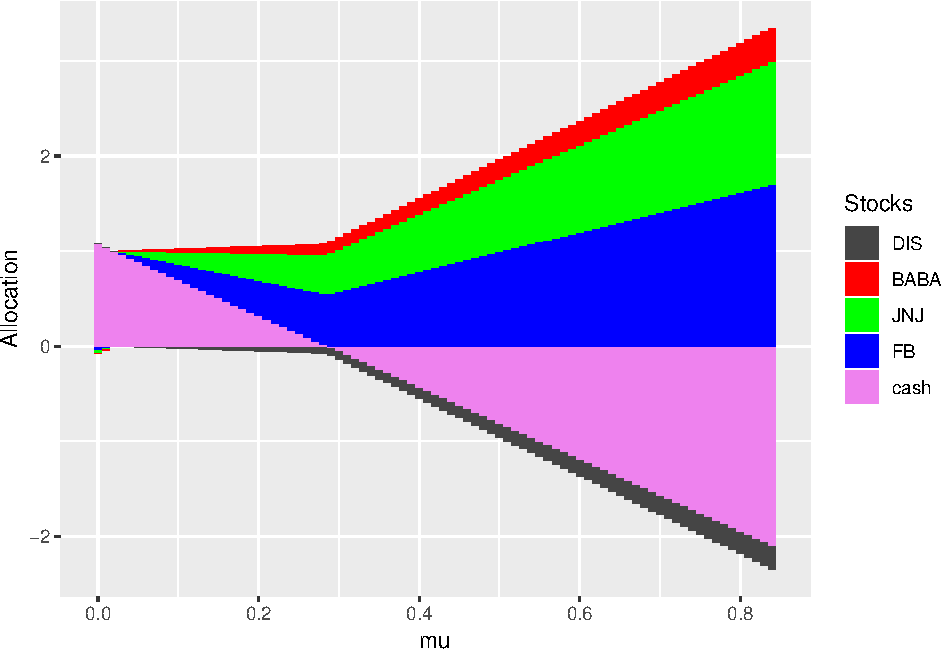
\includegraphics{Markowitz_Research_Me_files/figure-latex/unnamed-chunk-23-2.pdf}

\paragraph{numerical solution for our problem with risk free
asset}\label{numerical-solution-for-our-problem-with-risk-free-asset}

\begin{Shaded}
\begin{Highlighting}[]
\NormalTok{(mu.ret <-}\StringTok{ }\NormalTok{returns)}
\end{Highlighting}
\end{Shaded}

\begin{verbatim}
##       DIS      BABA       JNJ        FB 
## 0.1005307 0.2686097 0.1532568 0.3612616
\end{verbatim}

\begin{Shaded}
\begin{Highlighting}[]
\NormalTok{r0 =}\StringTok{ }\FloatTok{0.02}
\NormalTok{(}\DataTypeTok{a =} \KeywordTok{as.numeric}\NormalTok{(mu.ret}\OperatorTok\StringTok{ }\NormalTok{inv_C }\OperatorTok\StringTok{ }\NormalTok{mu.ret))}
\end{Highlighting}
\end{Shaded}

\begin{verbatim}
## [1] 0.005081476
\end{verbatim}

\begin{Shaded}
\begin{Highlighting}[]
\NormalTok{(}\DataTypeTok{b =} \KeywordTok{as.numeric}\NormalTok{(mu.ret}\OperatorTok\StringTok{ }\NormalTok{inv_C }\OperatorTok\StringTok{ }\NormalTok{ones ))}
\end{Highlighting}
\end{Shaded}

\begin{verbatim}
## [1] 0.01892006
\end{verbatim}

\begin{Shaded}
\begin{Highlighting}[]
\NormalTok{(}\DataTypeTok{c =} \KeywordTok{as.numeric}\NormalTok{(ones }\OperatorTok\StringTok{ }\NormalTok{inv_C }\OperatorTok\StringTok{ }\NormalTok{ones ))}
\end{Highlighting}
\end{Shaded}

\begin{verbatim}
## [1] 0.1178991
\end{verbatim}

\begin{Shaded}
\begin{Highlighting}[]
\NormalTok{(}\DataTypeTok{d =}\NormalTok{ a}\OperatorTok{-}\DecValTok{2}\OperatorTok{*}\NormalTok{b}\OperatorTok{*}\NormalTok{r0}\OperatorTok{+}\NormalTok{c}\OperatorTok{*}\NormalTok{r0}\OperatorTok{*}\NormalTok{r0)}
\end{Highlighting}
\end{Shaded}

\begin{verbatim}
## [1] 0.004371833
\end{verbatim}

\begin{Shaded}
\begin{Highlighting}[]
\NormalTok{(}\DataTypeTok{mu_0 =}\NormalTok{ (a }\OperatorTok{-}\StringTok{ }\NormalTok{b}\OperatorTok{*}\NormalTok{r0)}\OperatorTok{/}\NormalTok{(b}\OperatorTok{-}\NormalTok{c}\OperatorTok{*}\NormalTok{r0))}
\end{Highlighting}
\end{Shaded}

\begin{verbatim}
## [1] 0.2839664
\end{verbatim}

\begin{Shaded}
\begin{Highlighting}[]
\NormalTok{denominator <-}\StringTok{ }\NormalTok{r0 }\OperatorTok{-}\StringTok{ }\NormalTok{mu_}\DecValTok{0}
\NormalTok{sol_risky <-}\StringTok{ }\NormalTok{(}\DecValTok{1}\OperatorTok{/}\NormalTok{(b}\OperatorTok{-}\NormalTok{r0}\OperatorTok{*}\NormalTok{c))}\OperatorTok{*}\NormalTok{((inv_C }\OperatorTok\StringTok{ }\NormalTok{returns) }\OperatorTok{-}\StringTok{ }\NormalTok{(r0 }\OperatorTok{*}\StringTok{ }\NormalTok{inv_C }\OperatorTok\StringTok{ }\NormalTok{ones))}
\NormalTok{sol_risky}
\end{Highlighting}
\end{Shaded}

\begin{verbatim}
##             [,1]
## DIS  -0.07655683
## BABA  0.11422041
## JNJ   0.41668814
## FB    0.54564828
\end{verbatim}


\end{document}
